\begin{frame}{}
    \LARGE SSL: \textbf{Pretext Task Taxonomy}
\end{frame}

\begin{frame}[allowframebreaks]{Pretext Task Taxonomy: Introduction}
    \textbf{Pretext tasks} are broadly categorized by their supervision signal and learning objective: 
    \begin{itemize}
        \item \textbf{Reconstructive Methods}: Focus on reconstructing parts or properties of the input data.
        \item \textbf{Predictive Methods}: Involve predicting withheld or transformed aspects of the data.
    \end{itemize}
    
    Each category includes various techniques that have advanced SSL in computer vision.
    
    Understanding this taxonomy helps in:
    \begin{itemize}
        \item Selecting suitable pretext tasks for specific applications.
        \item Gaining insight into how SSL methods learn robust and transferable representations.
    \end{itemize}
\end{frame}

% \begin{frame}[allowframebreaks]{Denoising Autoencoders}
    \begin{itemize}
        \item \textbf{Corrupt input:} Introduce random noise to the input data, such as masking or adding Gaussian noise. The autoencoder is then trained to reconstruct the original, clean input from the corrupted version.
        \item \textbf{Robust feature learning:} By learning to recover the original data, the autoencoder is encouraged to extract meaningful and robust features that are less sensitive to noise and irrelevant variations.
        \item \textbf{Incremental understanding:} This approach helps the model generalize better by preventing it from simply memorizing the input, thus improving its ability to handle unseen or noisy data.
    \end{itemize}

    \framebreak

    \begin{figure}
        \centering
        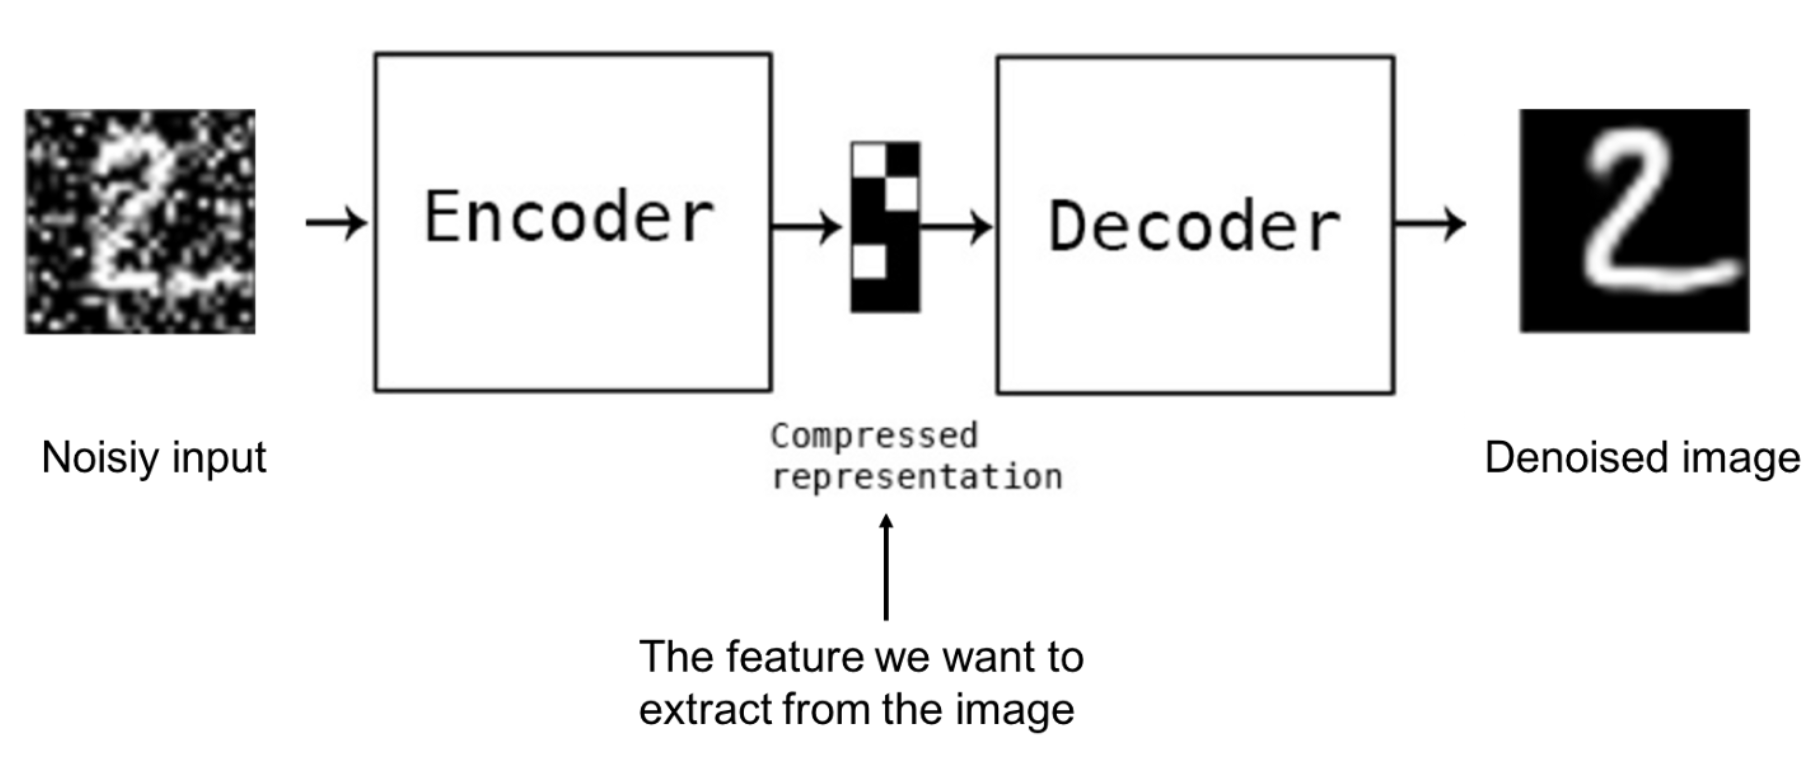
\includegraphics[width=\linewidth,height=0.9\textheight,keepaspectratio]{images/ssl/slide_12_1_img.png}
    \end{figure}

    \framebreak

    \begin{figure}
        \centering
        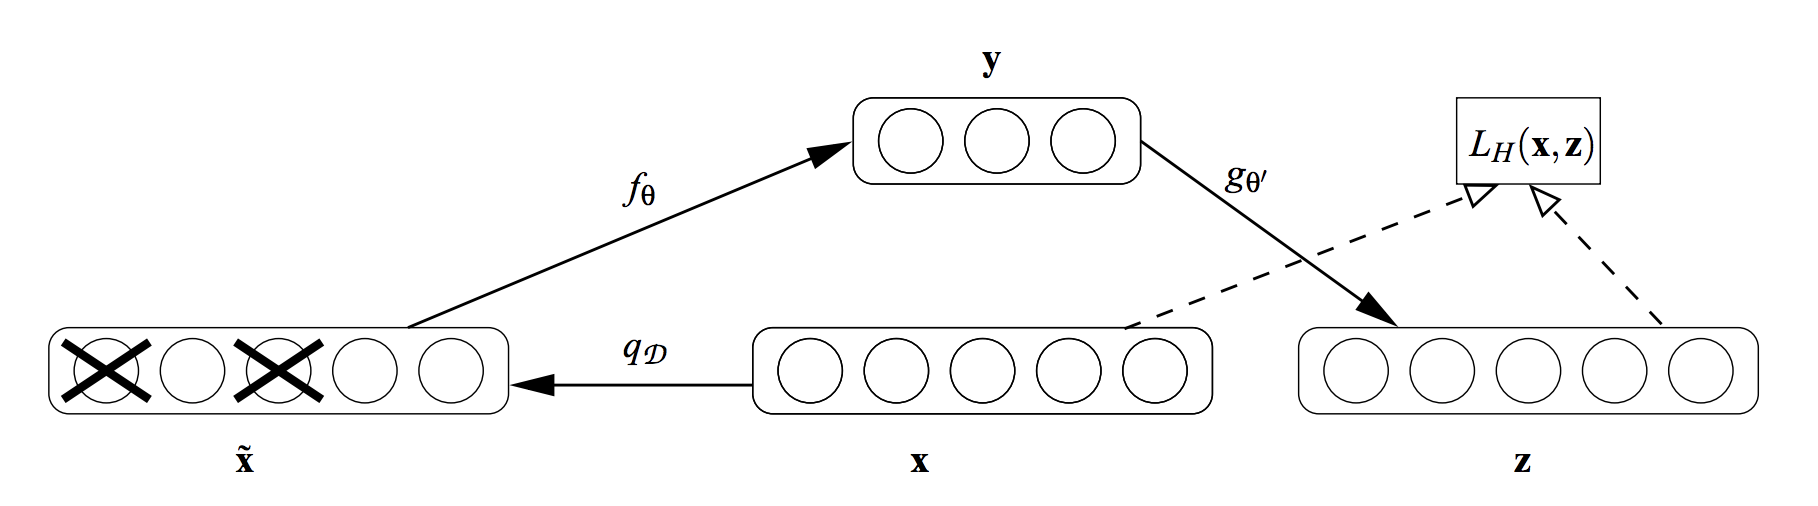
\includegraphics[width=\linewidth,height=0.9\textheight,keepaspectratio]{images/ssl/slide_13_1_img.png}
    \end{figure}

    \framebreak

    \begin{figure}
        \flushleft
        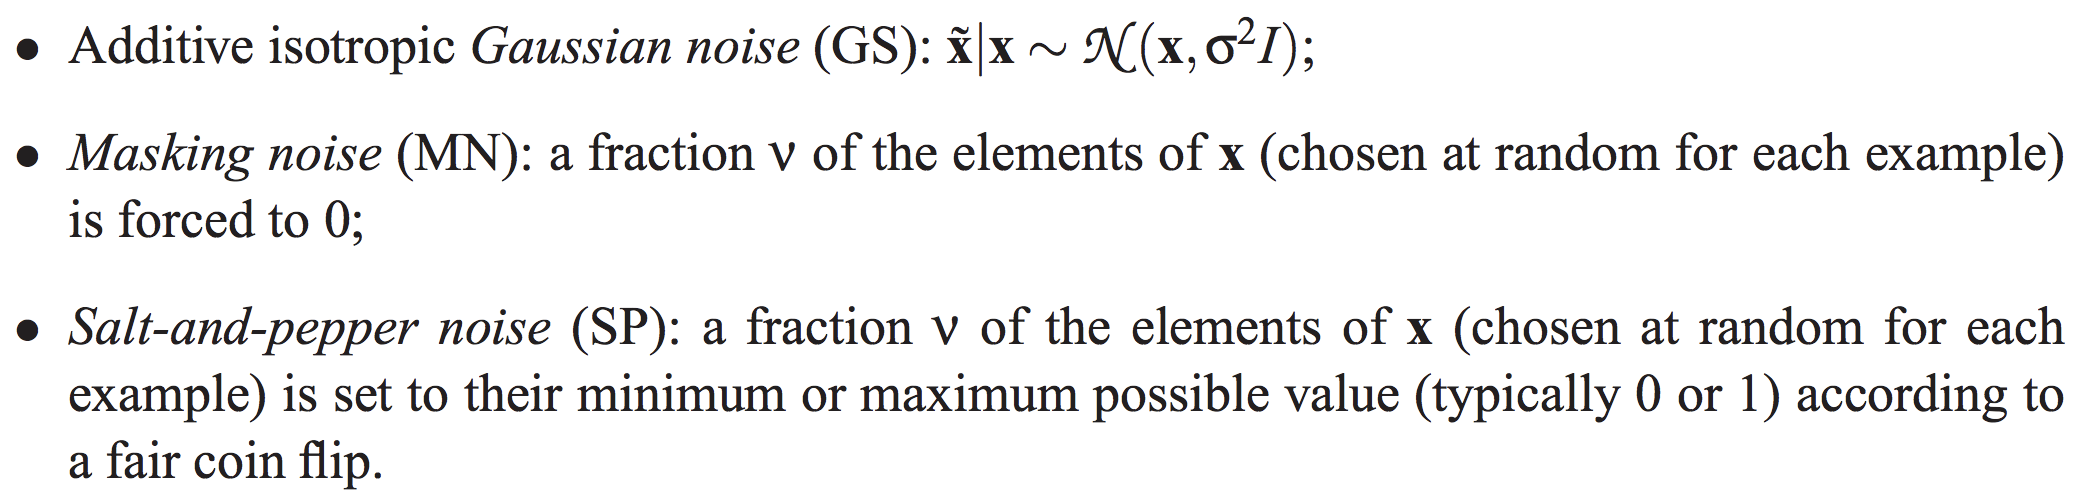
\includegraphics[width=1.08\linewidth,height=\textheight,keepaspectratio]{images/ssl/slide_14_1_img.png}
        \footnote{Vincent et al (2010). Denoising Autoencoders: Unsupervised Learning of Image Features from Noisy Data. ICML 2010.}
    \end{figure}
\end{frame}

\begin{frame}[allowframebreaks]{Emphasizing corrupted dimensions}
    \begin{figure}
        \flushleft
        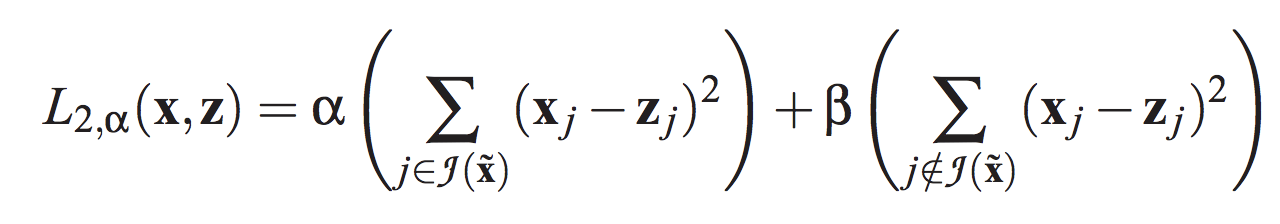
\includegraphics[width=1.08\linewidth,height=\textheight,keepaspectratio]{images/ssl/slide_15_1_img.png}
    \end{figure}

    \begin{figure}
        \flushleft
        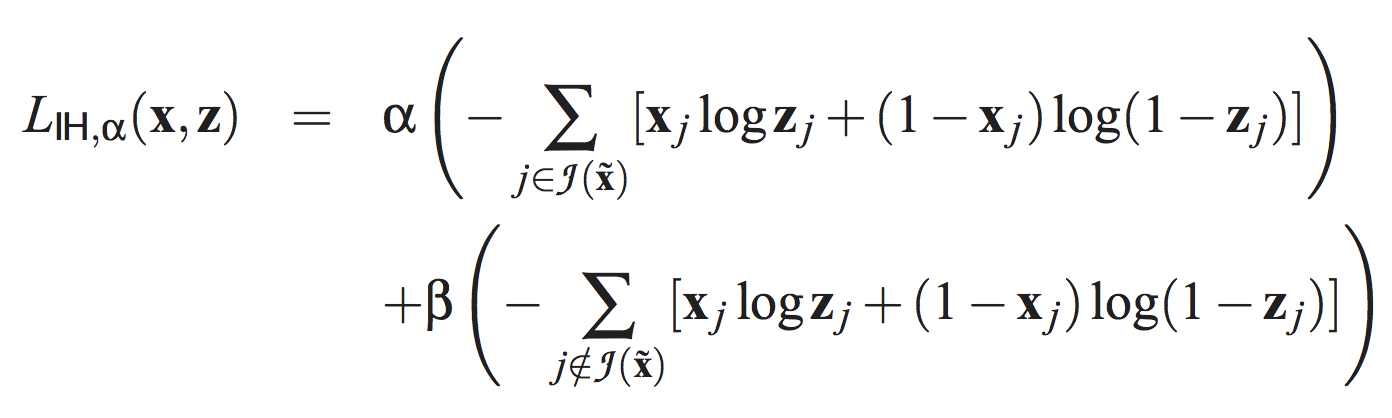
\includegraphics[width=1.08\linewidth,height=\textheight,keepaspectratio]{images/ssl/slide_15_2_img.png}
        \footnote{Vincent et al (2010). Denoising Autoencoders: Unsupervised Learning of Image Features from Noisy Data. ICML 2010.}
    \end{figure}
\end{frame}

\begin{frame}[allowframebreaks]{Denoising Autoencoders}
    \begin{figure}
        \flushleft
        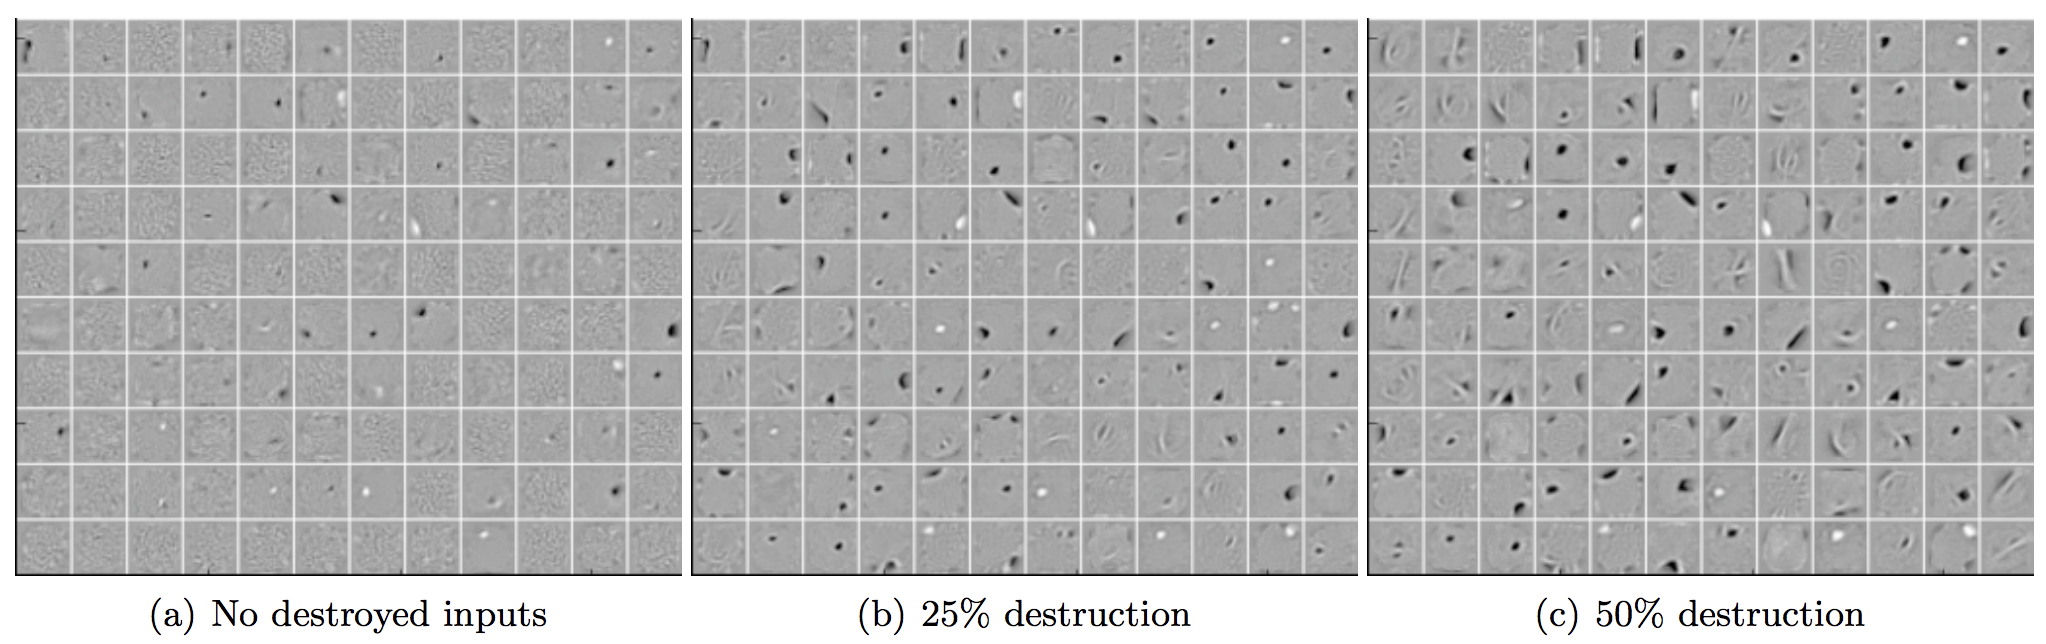
\includegraphics[width=1\linewidth,height=\textheight,keepaspectratio]{images/ssl/slide_16_1_img.png}
        \footnote{Vincent et al (2010). Denoising Autoencoders: Unsupervised Learning of Image Features from Noisy Data. ICML 2010.}
    \end{figure}
\end{frame}
% \begin{frame}[allowframebreaks]{Predict missing pieces}
    \begin{figure}
        \flushleft
        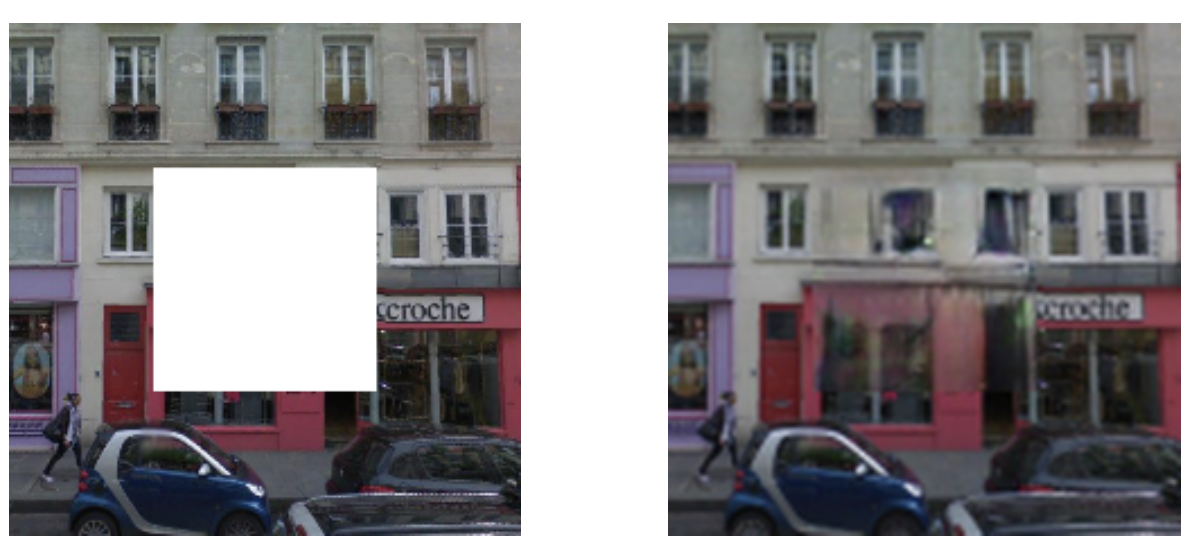
\includegraphics[width=1\linewidth,height=\textheight,keepaspectratio]{images/ssl/slide_17_1_img.png}
        \footnote{Pathak et al. (2016), "Context Encoders: Feature Learning by Inpainting," CVPR 2016.}
    \end{figure}
\end{frame}


\begin{frame}[allowframebreaks]{Context Encoders}
    \textbf{Context Encoders} are designed to learn meaningful image representations by reconstructing missing parts of an image.

    \vspace{0.15em}
    \textbf{Key Idea:}
    \begin{itemize}
        \setlength{\itemsep}{-0.5em}
        \item Randomly mask or remove patches from an input image.
        \item Use an encoder–decoder neural network to predict and reconstruct the missing content.
        \item The model is trained to minimize the difference between the predicted and actual image patches.
    \end{itemize}

    \vspace{0.15em}
    \textbf{Architecture:}
    \begin{itemize}
        \setlength{\itemsep}{-0.5em}
        \item \textbf{Encoder:} Processes the visible parts of the image and extracts feature representations.
        \item \textbf{Decoder:} Generates the missing image regions based on the encoded features.
        \item The entire network is trained end-to-end using a reconstruction loss (e.g., L2 loss).
    \end{itemize}

    \framebreak

    \begin{figure}
        \flushleft
        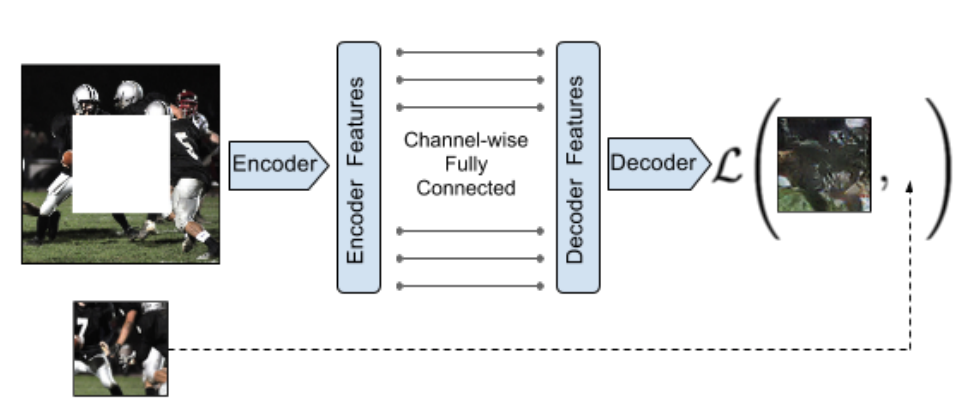
\includegraphics[width=1\linewidth,height=\textheight,keepaspectratio]{images/ssl/slide_18_1_img.png}
    \end{figure}

    \framebreak

    \begin{figure}
        \flushleft
        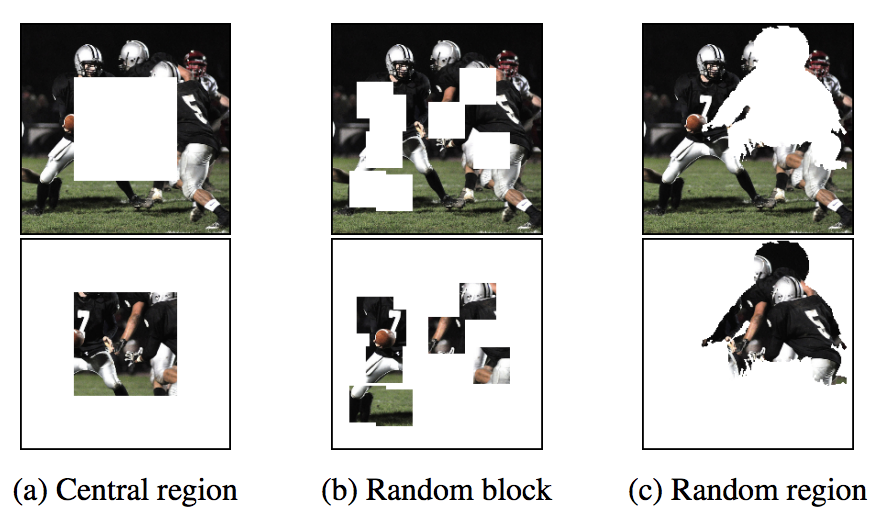
\includegraphics[width=1\linewidth,height=\textheight,keepaspectratio]{images/ssl/slide_19_1_img.png}
    \end{figure}

    \framebreak

    \begin{figure}
        \flushleft
        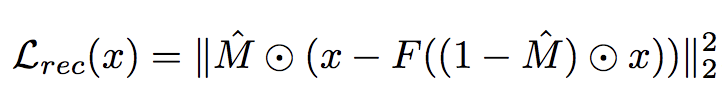
\includegraphics[width=1\linewidth,height=\textheight,keepaspectratio]{images/ssl/slide_20_3_img.png}
    \end{figure}

    \begin{figure}
        \flushleft
        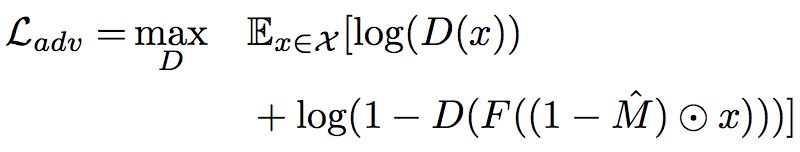
\includegraphics[width=1\linewidth,height=\textheight,keepaspectratio]{images/ssl/slide_20_2_img.png}
    \end{figure}

    \begin{figure}
        \centering
        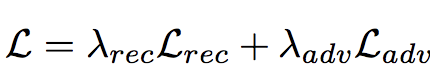
\includegraphics[width=0.7\linewidth,height=\textheight,keepaspectratio]{images/ssl/slide_20_1_img.png}
    \end{figure}

    \framebreak

    \begin{figure}
        \flushleft
        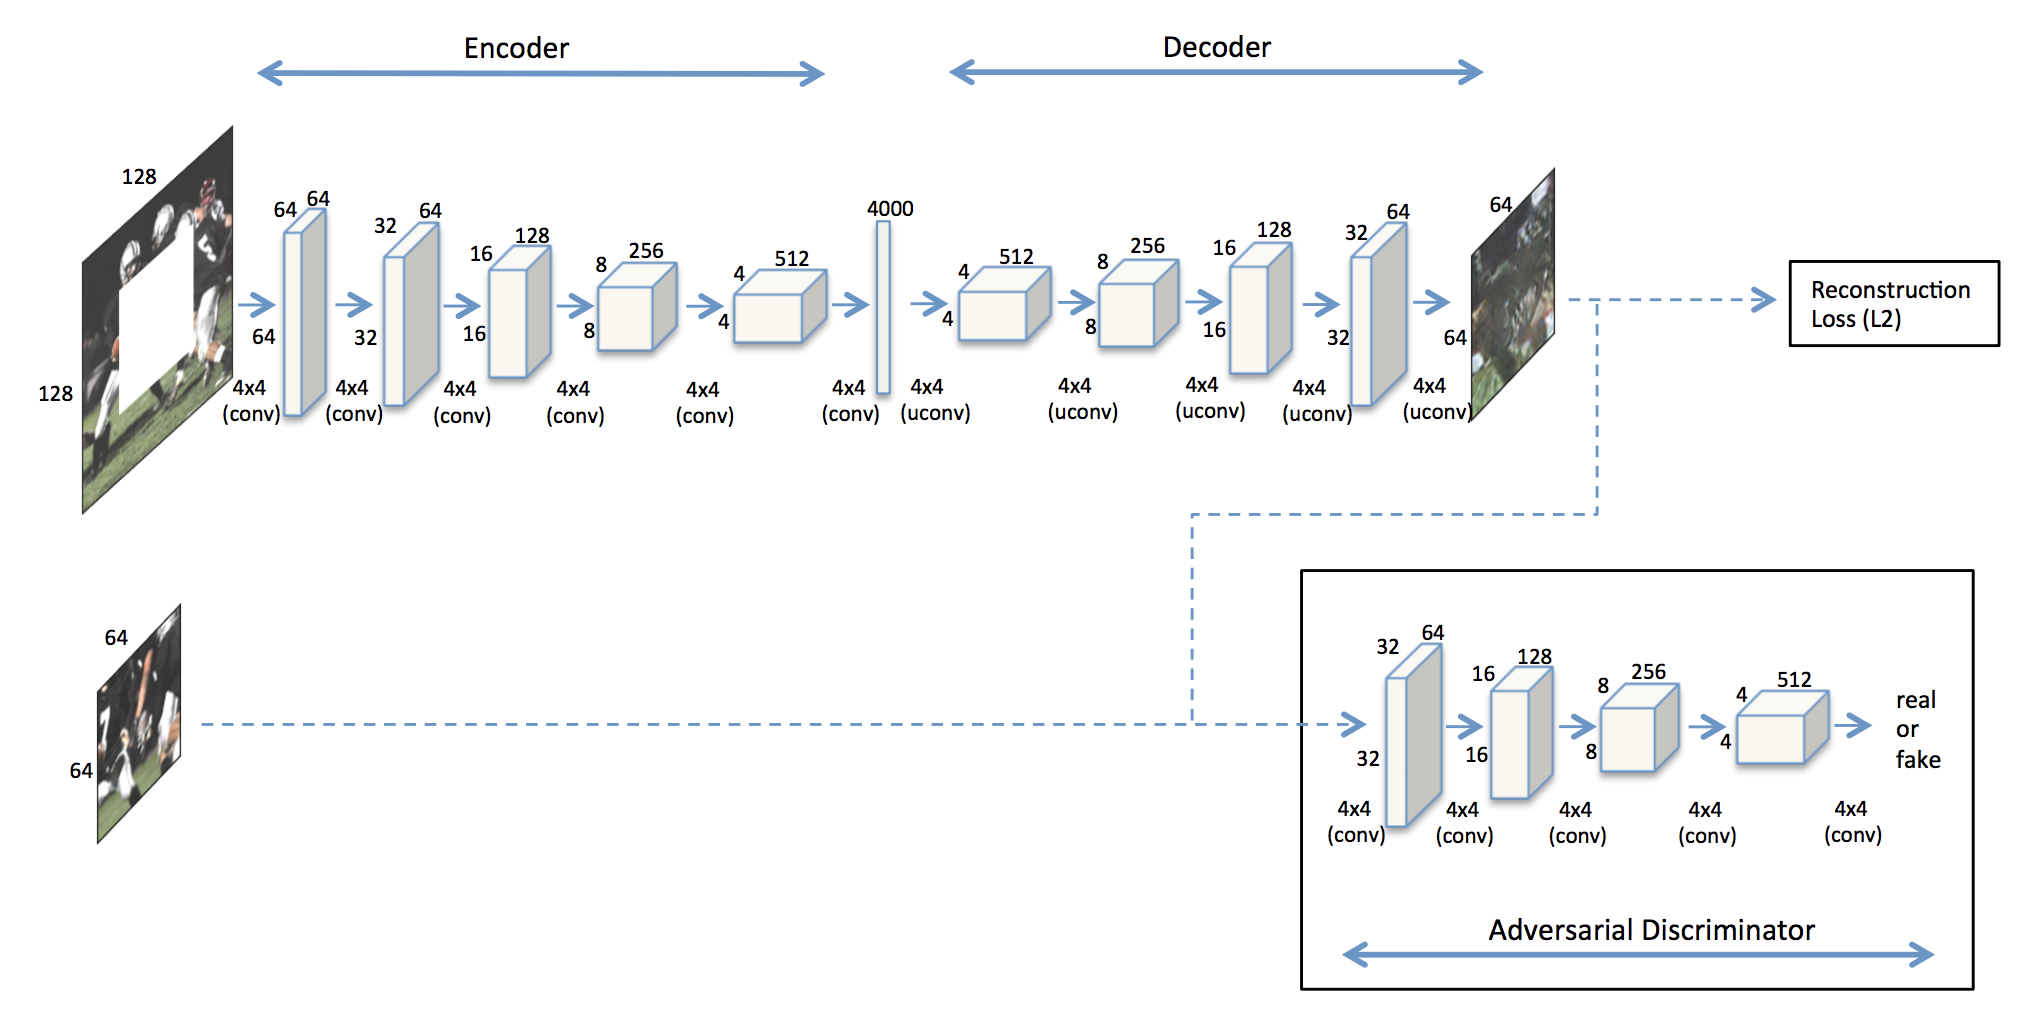
\includegraphics[width=1\linewidth,height=\textheight,keepaspectratio]{images/ssl/slide_21_1_img.png}
    \end{figure}

    \framebreak

    \begin{figure}
        \flushleft
        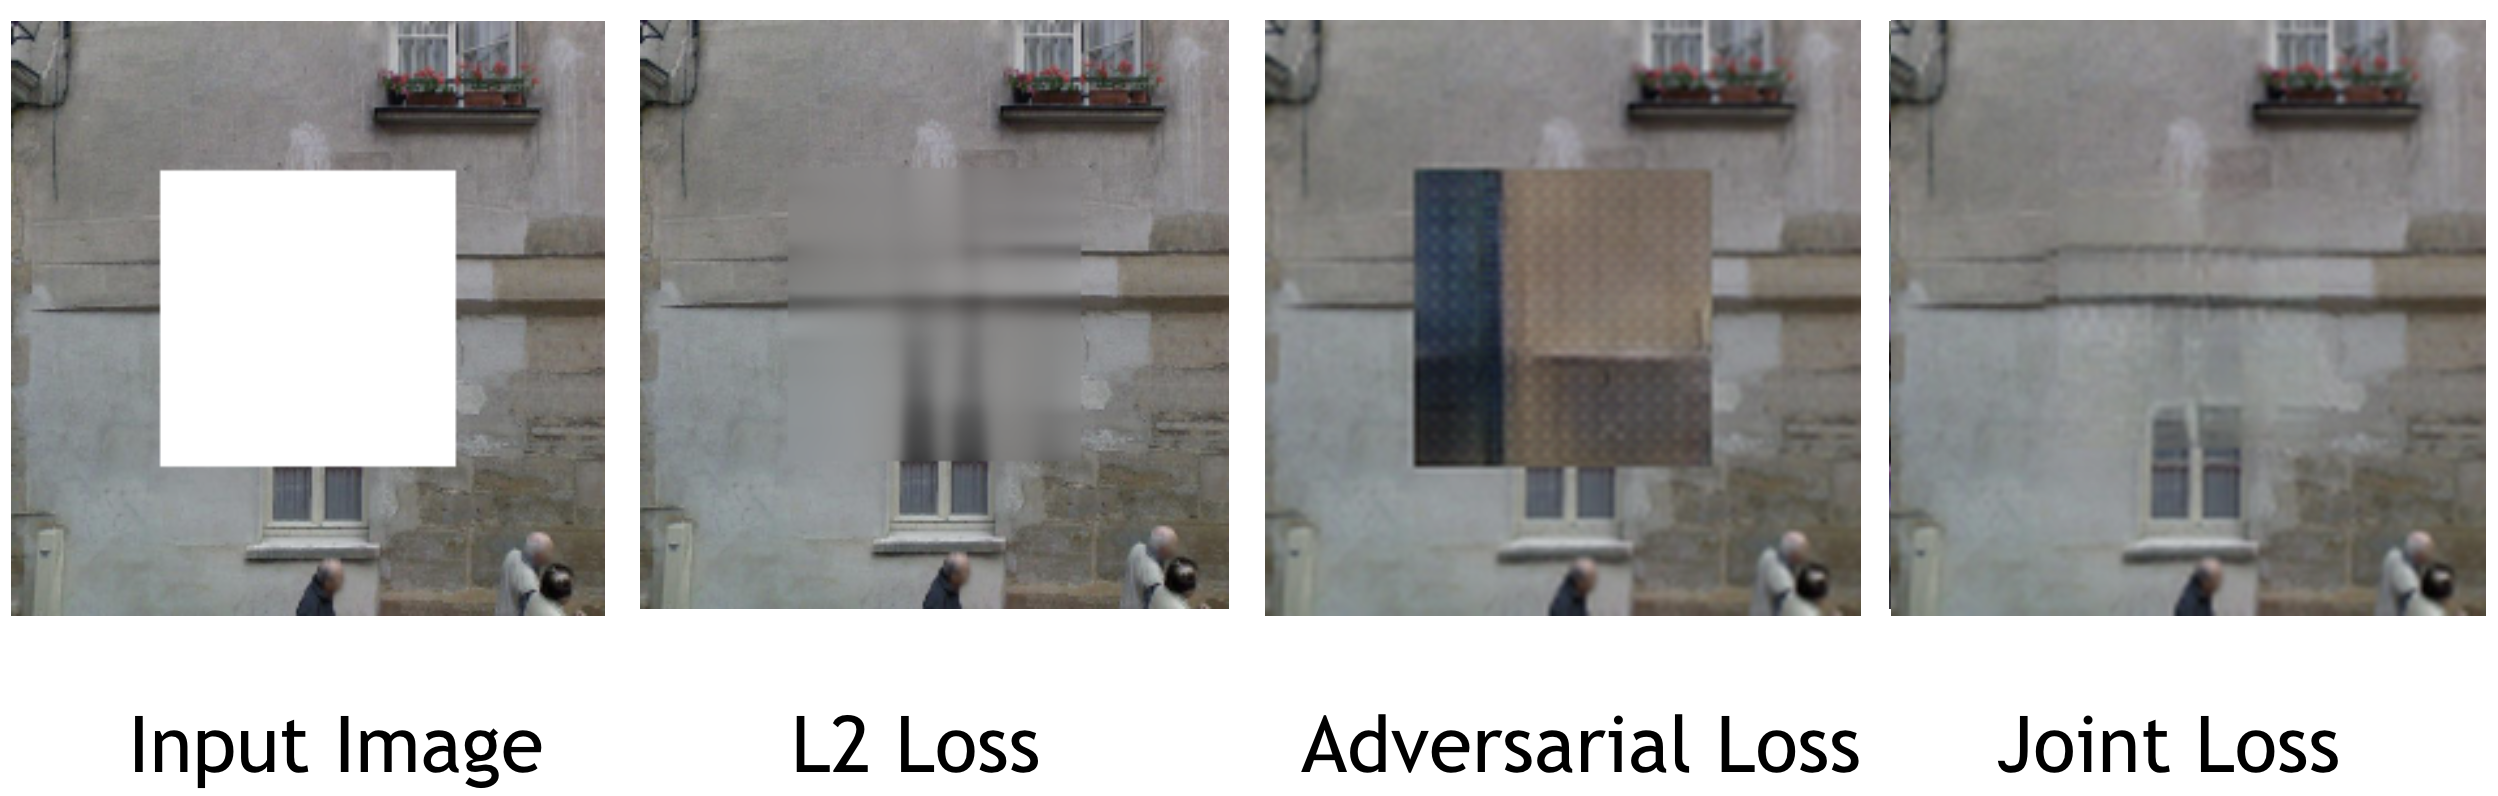
\includegraphics[width=1\linewidth,height=\textheight,keepaspectratio]{images/ssl/slide_22_1_img.png}
    \end{figure}

    \framebreak

    \begin{figure}
        \flushleft
        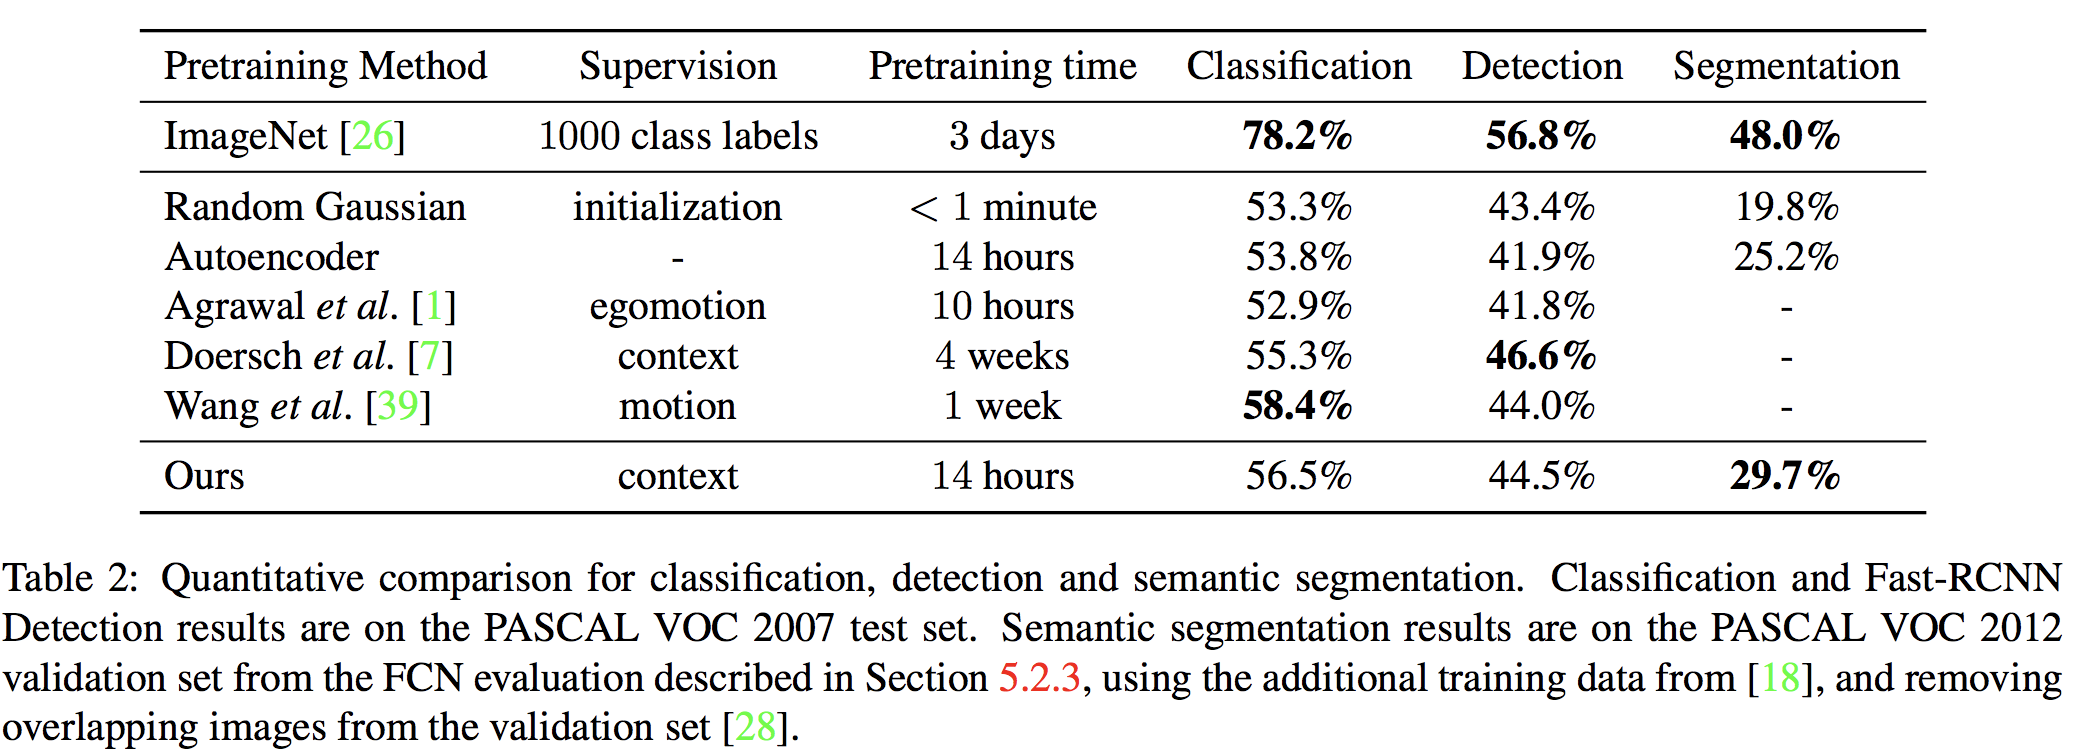
\includegraphics[width=1\linewidth,height=\textheight,keepaspectratio]{images/ssl/slide_23_1_img.png}
    \end{figure}

    \framebreak

    \vspace{0.5em}
    \textbf{Why does this work?}
    \begin{itemize}
        \setlength{\itemsep}{-0.25em}
        \item The network must understand the global and local context of the image to generate plausible content.
        \item This forces the model to learn semantic features and relationships within the image.
        \item The learned representations can be transferred to downstream tasks such as classification, detection, or segmentation.
    \end{itemize}

    \vspace{0.5em}
    \textbf{Applications:}
    \begin{itemize}
        \setlength{\itemsep}{-0.25em}
        \item Image inpainting
        \item Representation learning for transfer to other vision tasks
        \item Anomaly detection (by comparing predicted and actual content)
    \end{itemize}

    \vspace{0.5em}
    \textbf{Reference:}
    \begin{itemize}
        \item Pathak et al., "Context Encoders: Feature Learning by Inpainting," CVPR 2016.
    \end{itemize}
\end{frame}
% \begin{frame}[allowframebreaks]{Predicting One View from Another}

    \textbf{Learn to translate between modalities or augmentations}
    \begin{itemize}
        \item The core idea is to train a model that can predict or reconstruct one view of the data given another.
        \item Views can be different modalities (e.g., infrared vs. RGB), or different augmentations (e.g., color vs. grayscale, rotated images, etc.).
        \item This approach encourages the model to learn shared representations that capture the underlying semantics of the data, rather than superficial features.
    \end{itemize}

    \framebreak

    \begin{figure}
        \flushleft
        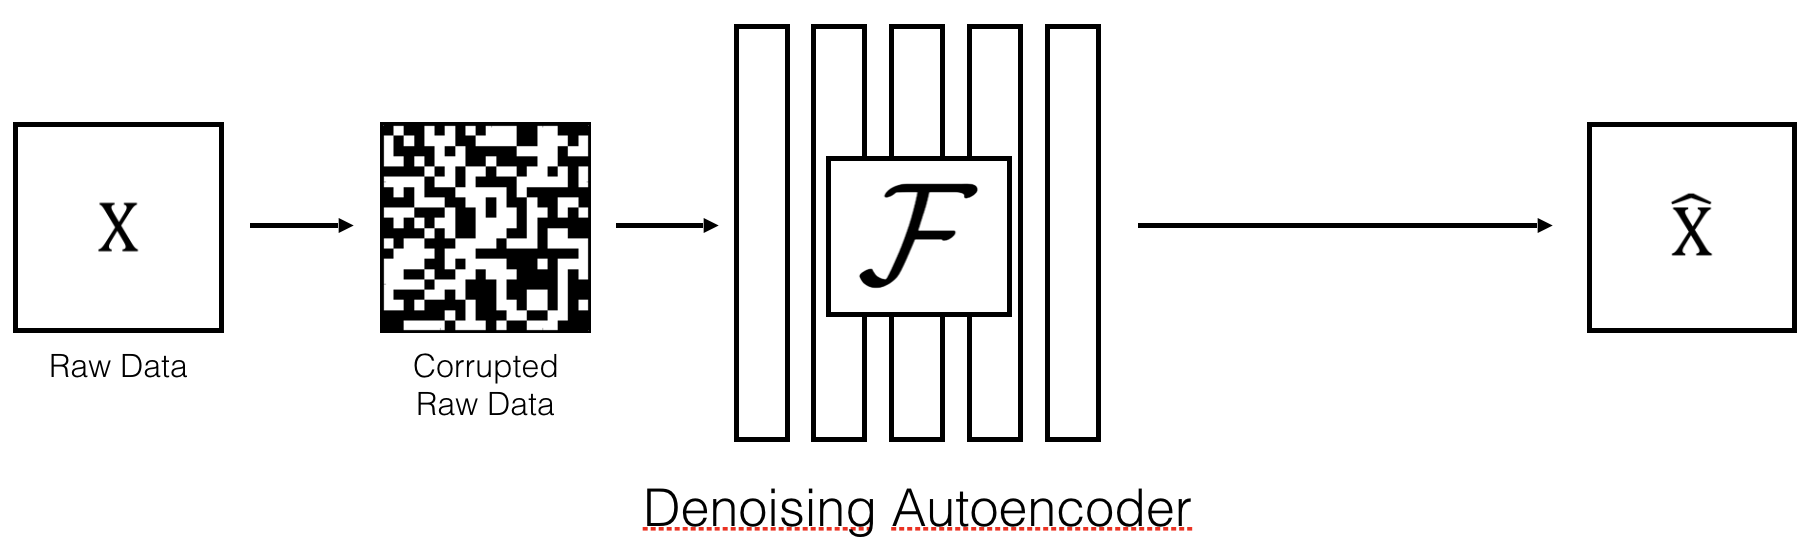
\includegraphics[width=1\linewidth,height=\textheight,keepaspectratio]{images/ssl/slide_24_1_img.png}
        Slide: Richard Zhang (2019). Predicting One View from Another.
    \end{figure}

    \framebreak

    \begin{figure}
        \flushleft
        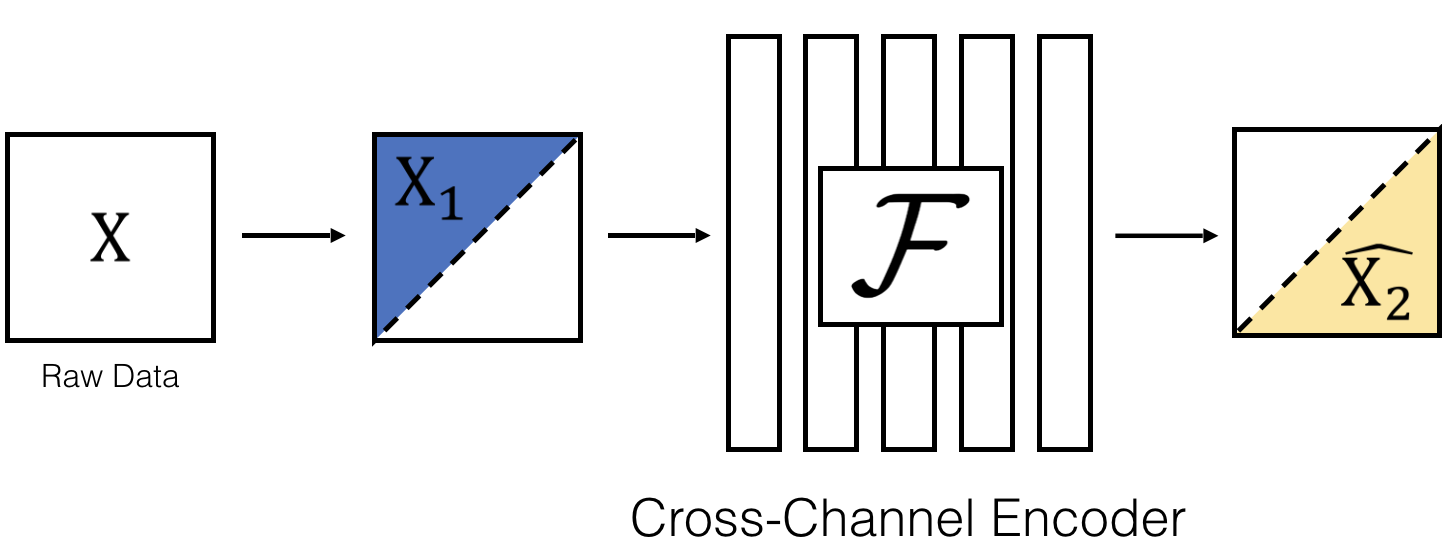
\includegraphics[width=1\linewidth,height=\textheight,keepaspectratio]{images/ssl/slide_25_1_img.png}
        Slide: Richard Zhang (2019). Predicting One View from Another.
    \end{figure}

    \framebreak

    \textbf{Example: Learn mapping from infrared to RGB imagery}
    \begin{itemize}
        \item In remote sensing, images are often captured in both infrared and RGB channels.
        \item A model can be trained to predict the RGB image given the infrared image, or vice versa.
        \item This task forces the model to understand the relationship between the two modalities, which can improve its generalization and robustness.
        \item Such cross-modal prediction is useful for applications where one modality may be missing or corrupted.
    \end{itemize}

    \framebreak

    \begin{figure}
        \flushleft
        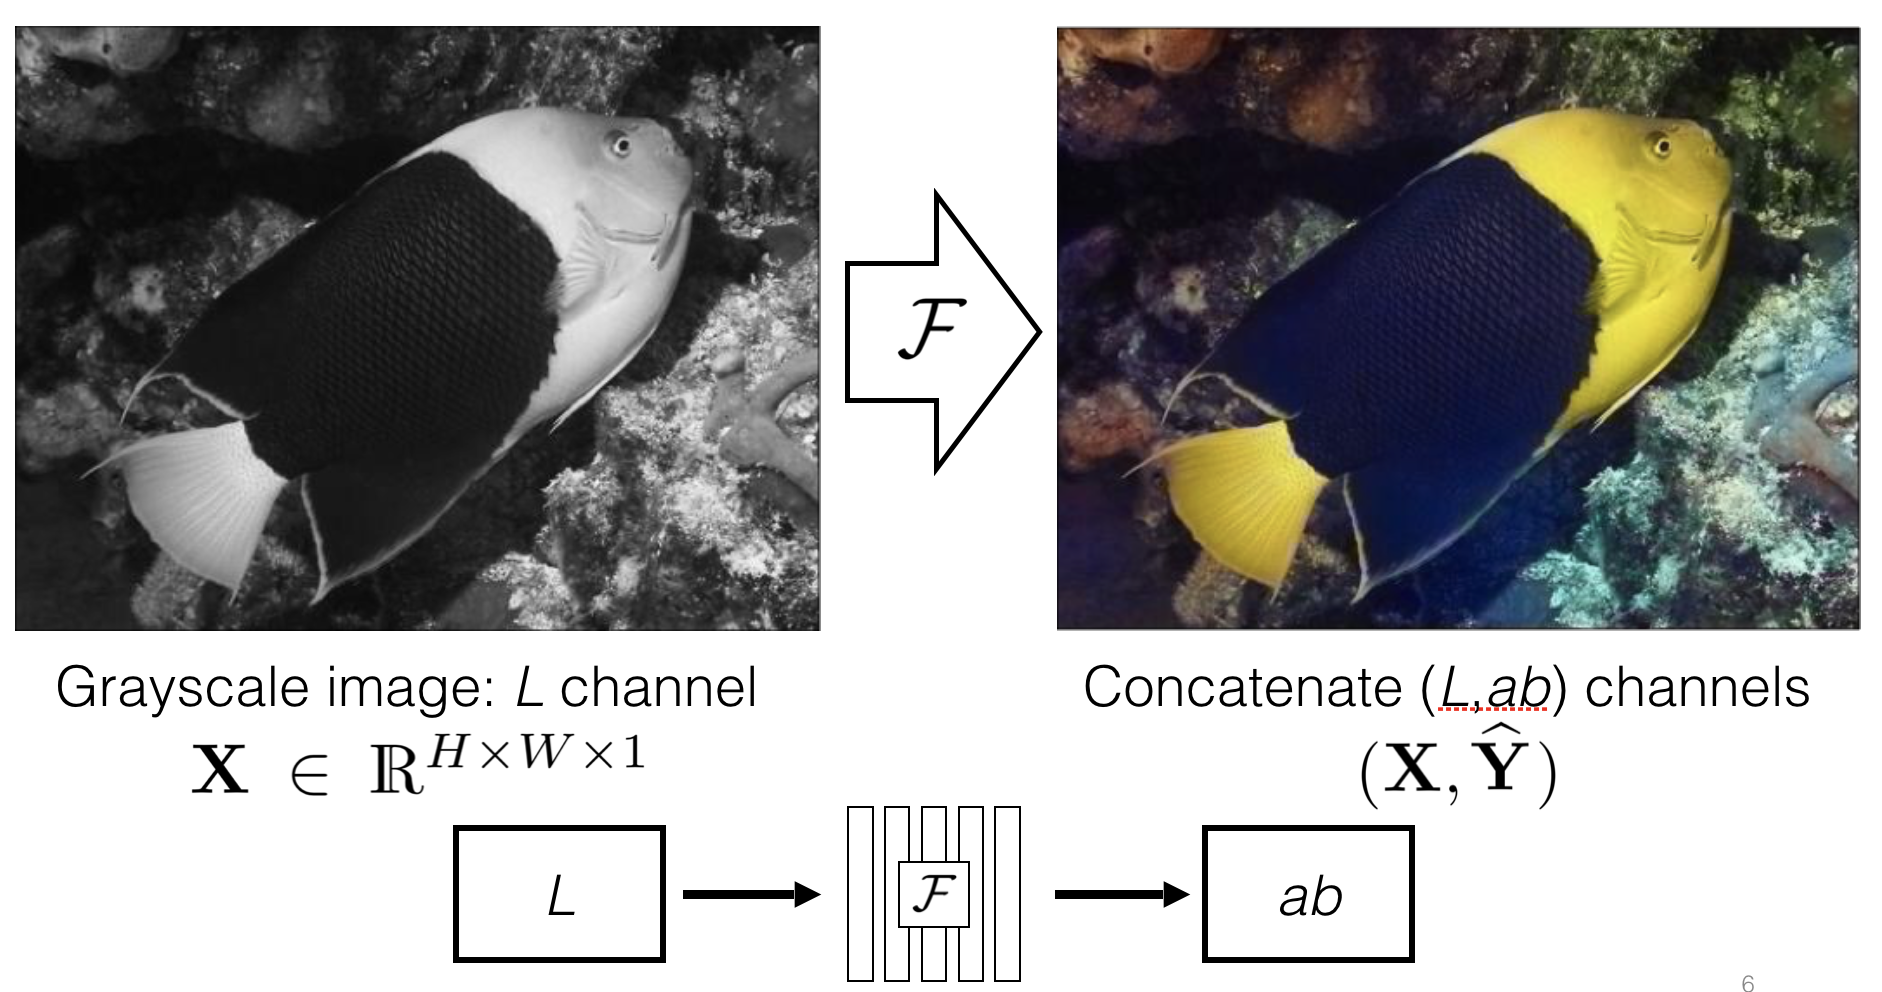
\includegraphics[width=1\linewidth,height=\textheight,keepaspectratio]{images/ssl/slide_26_1_img.png}
        Slide: Richard Zhang (2019). Predicting One View from Another.
    \end{figure}

    \framebreak

    \begin{figure}
        \flushleft
        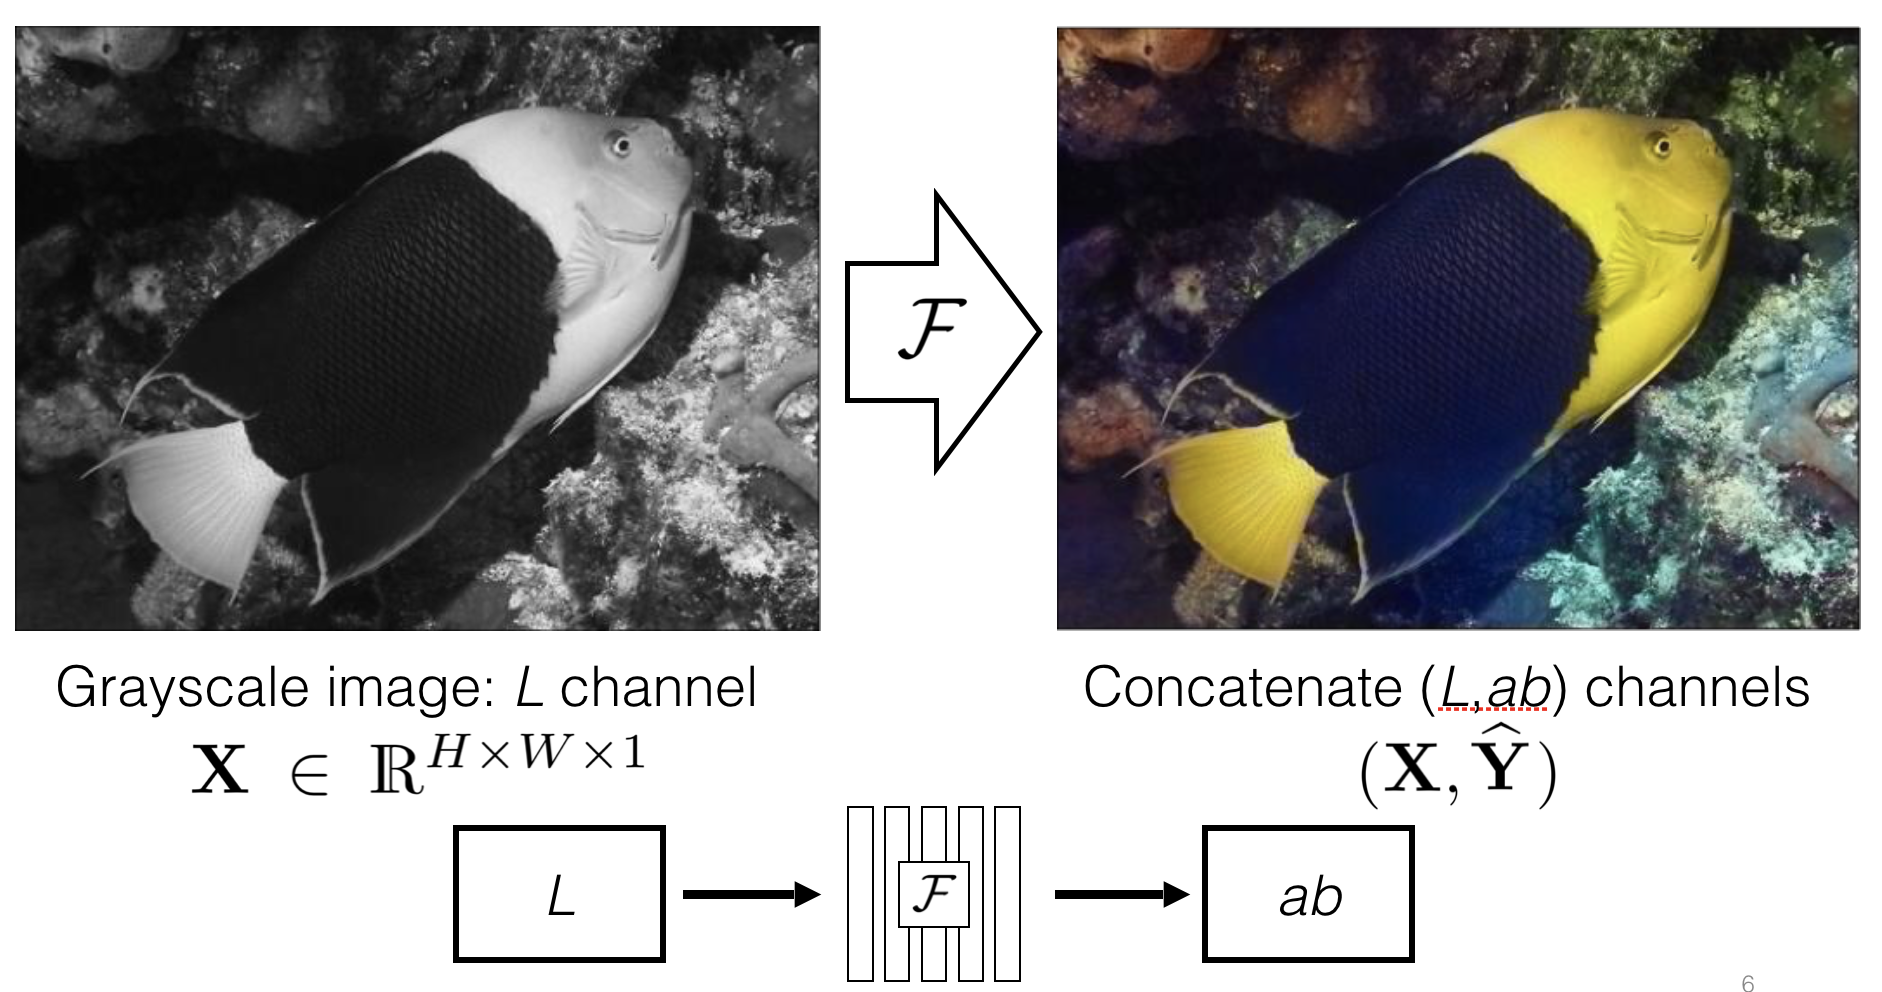
\includegraphics[width=1\linewidth,height=\textheight,keepaspectratio]{images/ssl/slide_27_1_img.png}
        Slide: Richard Zhang (2019). Predicting One View from Another.
    \end{figure}

    \framebreak

    \begin{figure}
        \flushleft
        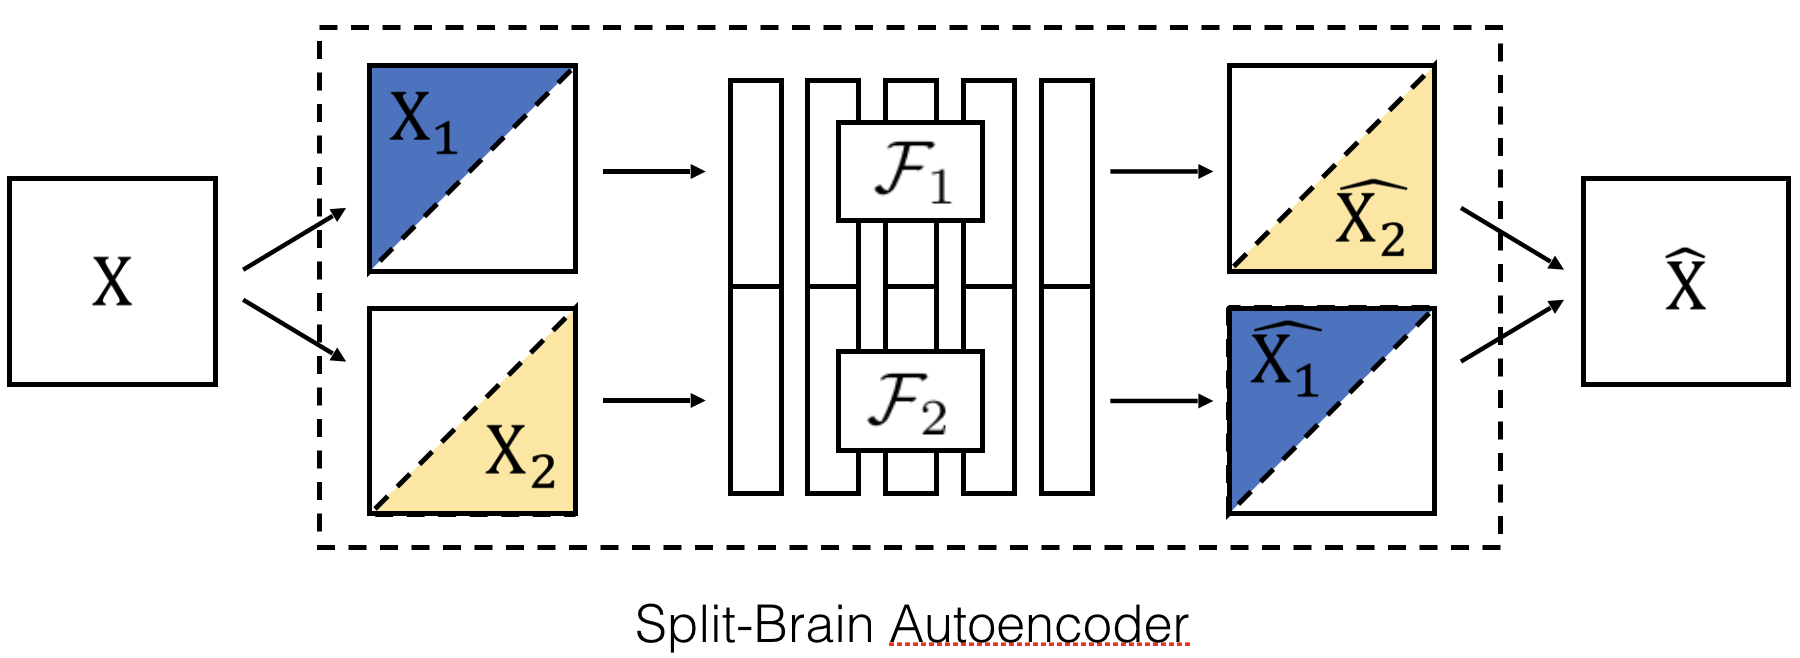
\includegraphics[width=1\linewidth,height=\textheight,keepaspectratio]{images/ssl/slide_28_1_img.png}
        Slide: Richard Zhang (2019). Predicting One View from Another.
    \end{figure}

    \framebreak
    
    \begin{itemize} 
        \item \textbf{Applications and Benefits}
        \begin{itemize}
            \item \textbf{Data augmentation}: By learning to predict one augmentation from another, models become more invariant to transformations.
            \item \textbf{Multi-modal learning}: Enables leveraging complementary information from different data sources.
            \item \textbf{Self-supervised learning}: No need for manual labels, as the prediction task itself provides the supervision.
        \end{itemize}
        \item \textbf{Challenges}
        \begin{itemize}
            \item The mapping between modalities may be complex and non-linear.
            \item Requires careful design of architectures and loss functions to ensure meaningful learning.
        \end{itemize}
    \end{itemize}

    
\end{frame}
% \begin{frame}[allowframebreaks]{Relative Position of Image Patches}
    \begin{figure}
        \centering
        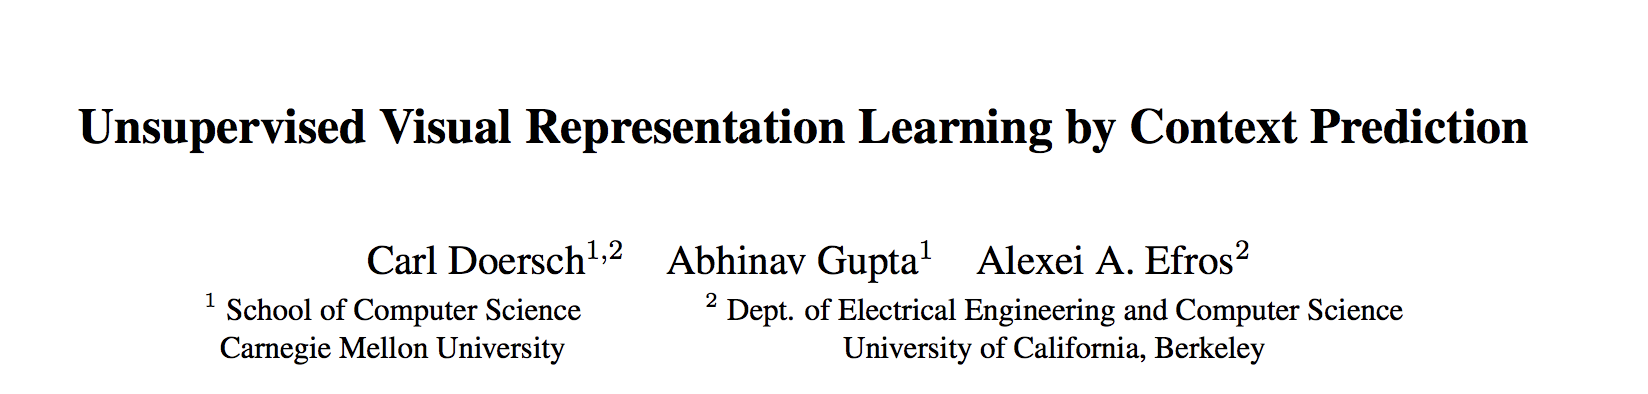
\includegraphics[width=1\linewidth,height=\textheight,keepaspectratio]{images/ssl/slide_29_2_img.png}
    \end{figure}
    \begin{figure}
        \centering
        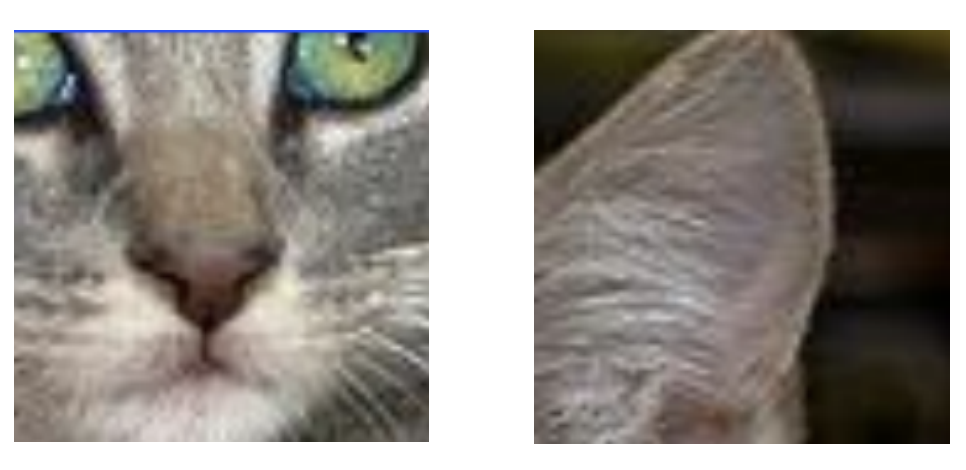
\includegraphics[width=0.5\linewidth,height=0.6\textheight,keepaspectratio]{images/ssl/slide_29_1_img.png}
        
        Slide: Zisserman et al (2019). Relative Position of Image Patches.
    \end{figure}

    \textbf{Task}: Predict the relative position of the second patch with respect to the first


    \framebreak

    \textbf{Shuffle image patches; predict their relative spatial positions.}
    \begin{itemize}
        \item The input image is divided into several non-overlapping patches.
        \item These patches are randomly shuffled to disrupt their original spatial arrangement.
        \item The model is tasked with predicting the original relative positions of the shuffled patches.
    \end{itemize}

    \framebreak

    \begin{figure}
        \centering
        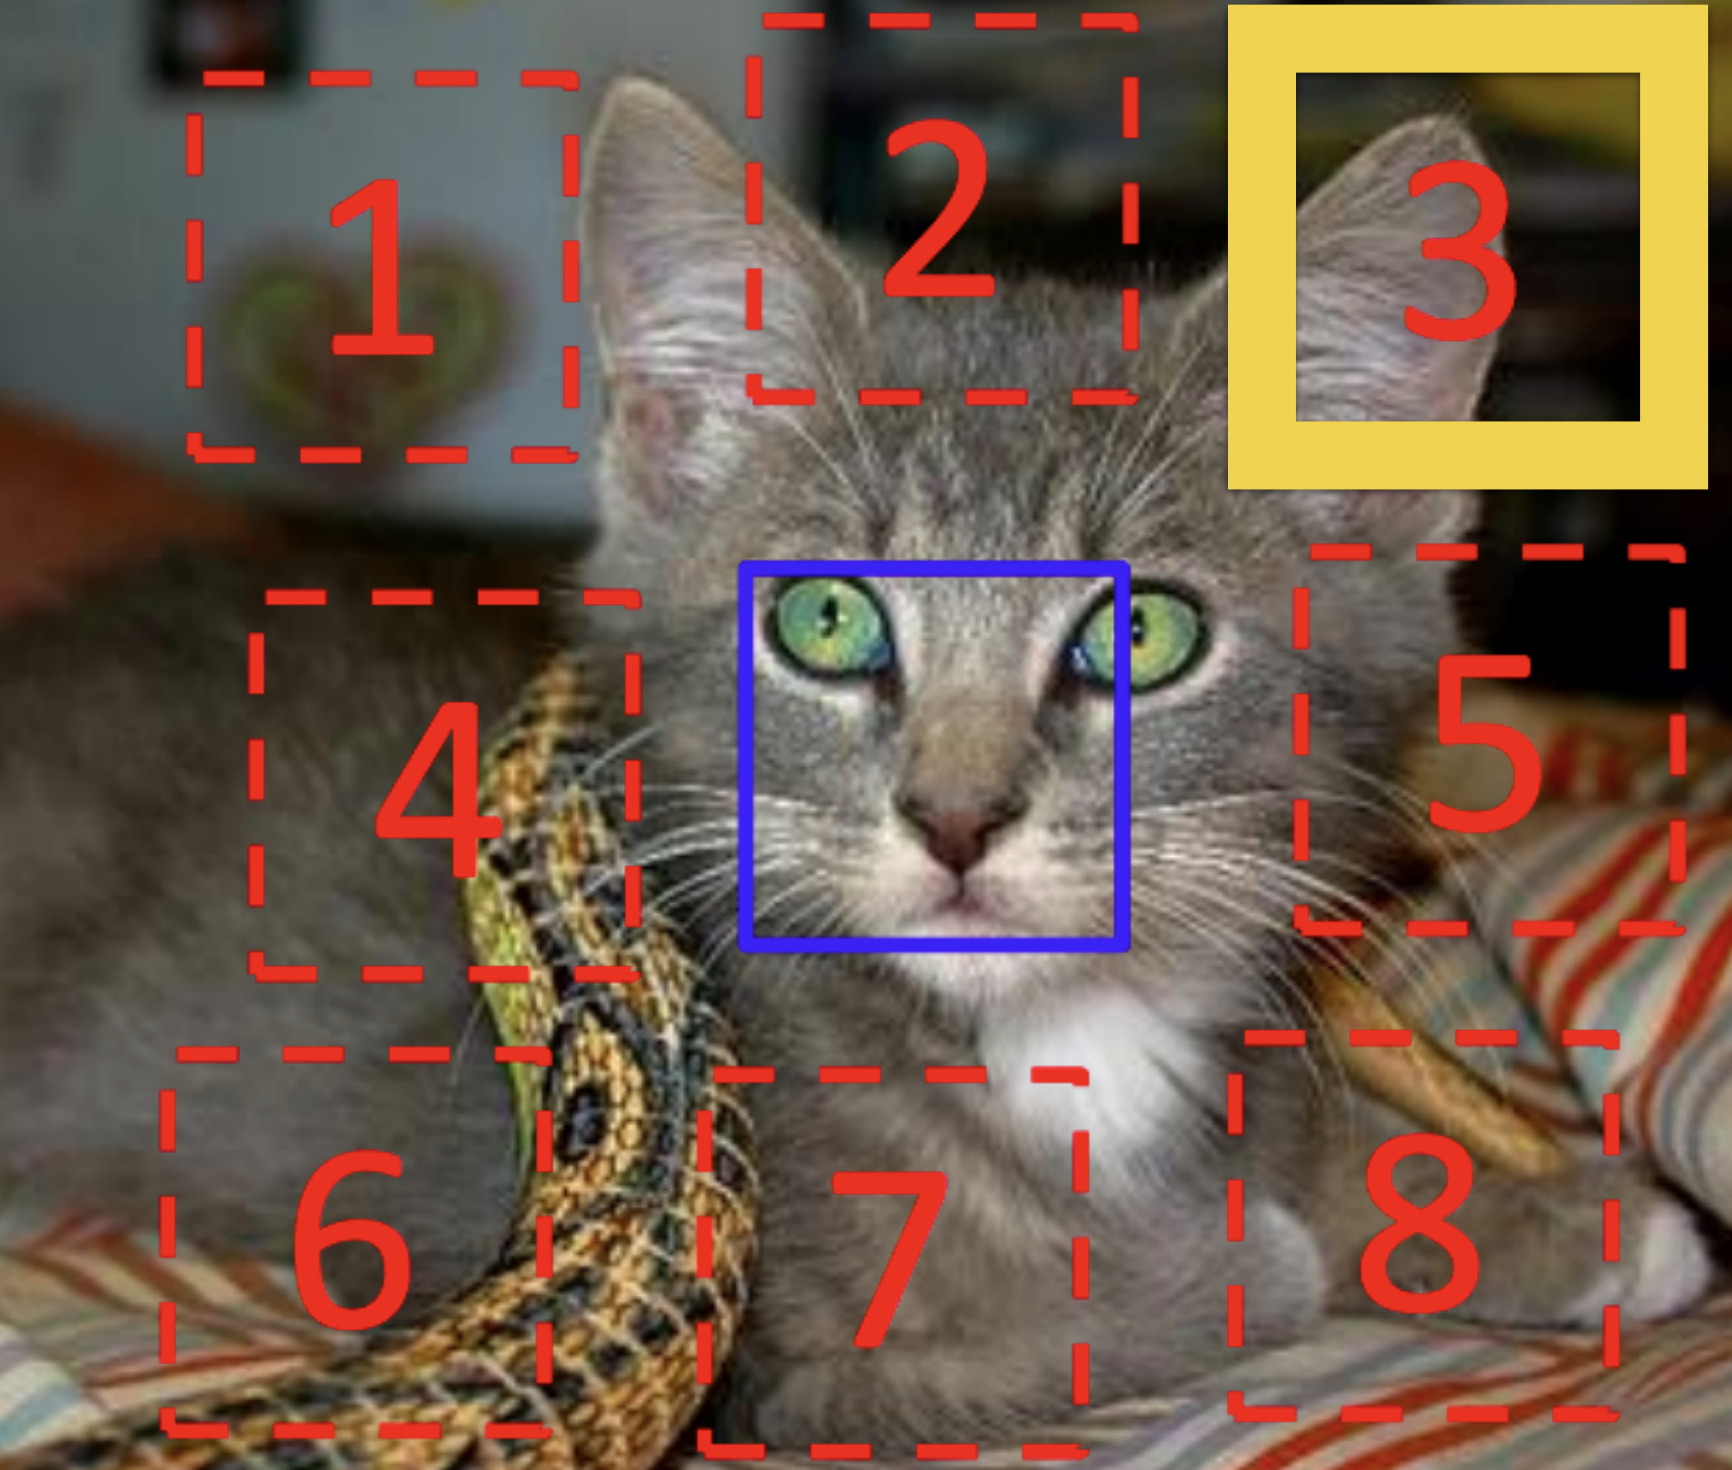
\includegraphics[width=\linewidth,height=0.9\textheight,keepaspectratio]{images/ssl/slide_30_1_img.png}
    \end{figure}

    \framebreak

    \begin{figure}
        \centering
        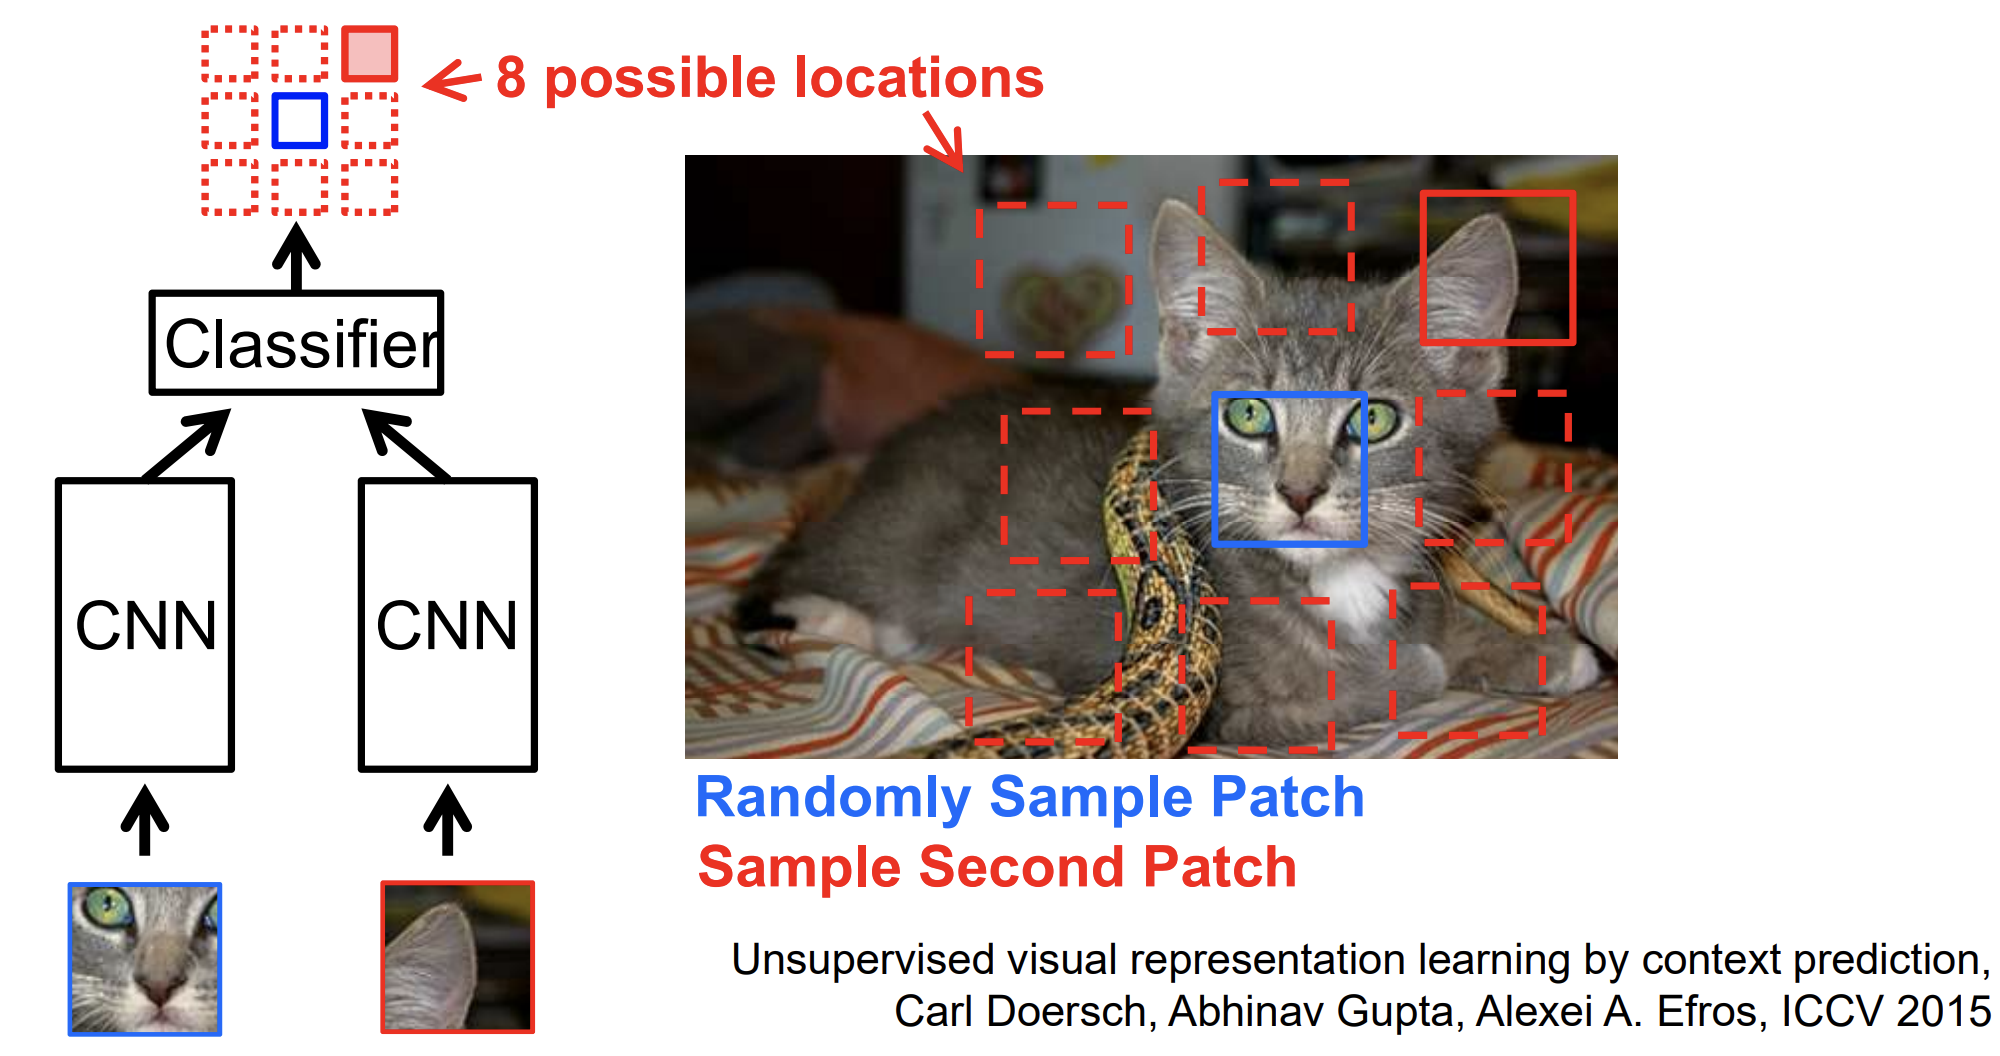
\includegraphics[width=\linewidth,height=0.9\textheight,keepaspectratio]{images/ssl/slide_31_1_img.png}
    \end{figure}

    \framebreak

    \textbf{Model learns geometric relationships and spatial context.}
    \begin{itemize}
        \item By solving the patch position prediction task, the model is forced to understand the underlying spatial structure of objects and scenes.
        \item This encourages the learning of features that capture geometric relationships between different parts of the image.
        \item Such self-supervised tasks help the model develop a strong sense of spatial context, which is beneficial for downstream vision tasks like object detection and segmentation.
    \end{itemize}

    \framebreak

    \textbf{Solving Jigsaw puzzles as a pretext task.}

    \begin{figure}
        \centering
        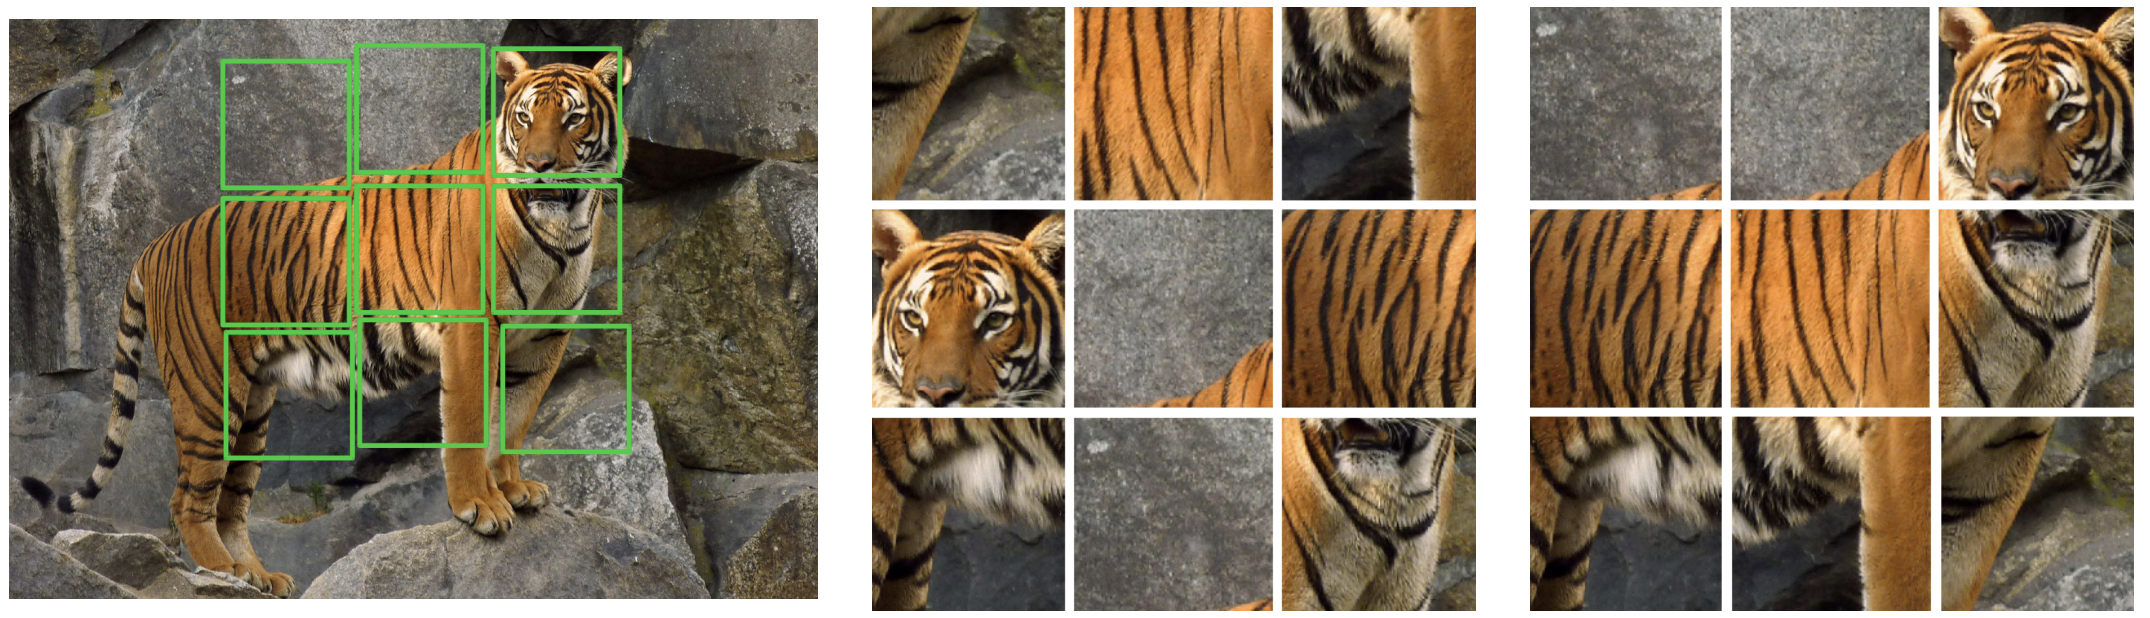
\includegraphics[width=\linewidth,height=0.9\textheight,keepaspectratio]{images/ssl/slide_32_1_img.png}
    \end{figure}
\end{frame}
% \begin{frame}[allowframebreaks]{Rotation Prediction}
    \textbf{Rotation Prediction} is commonly used to learn useful image representations without requiring manual labels.
    \begin{itemize}
        \item \textbf{Task:} Rotate input images by a set of predefined angles (e.g., $0^\circ$, $90^\circ$, $180^\circ$, $270^\circ$).
        \item \textbf{Objective:} Train a neural network to predict the rotation angle applied to each image.
        \item \textbf{Implementation Steps:}
        \begin{itemize}
            \item Randomly select a rotation angle from the set.
            \item Apply the rotation to the input image.
            \item Feed the rotated image into the network.
            \item Use a classification head to predict the rotation angle.
            \item Compute the loss (e.g., cross-entropy) and update the model.
        \end{itemize}
    \end{itemize}

    \framebreak

    \begin{figure}
        \flushleft
        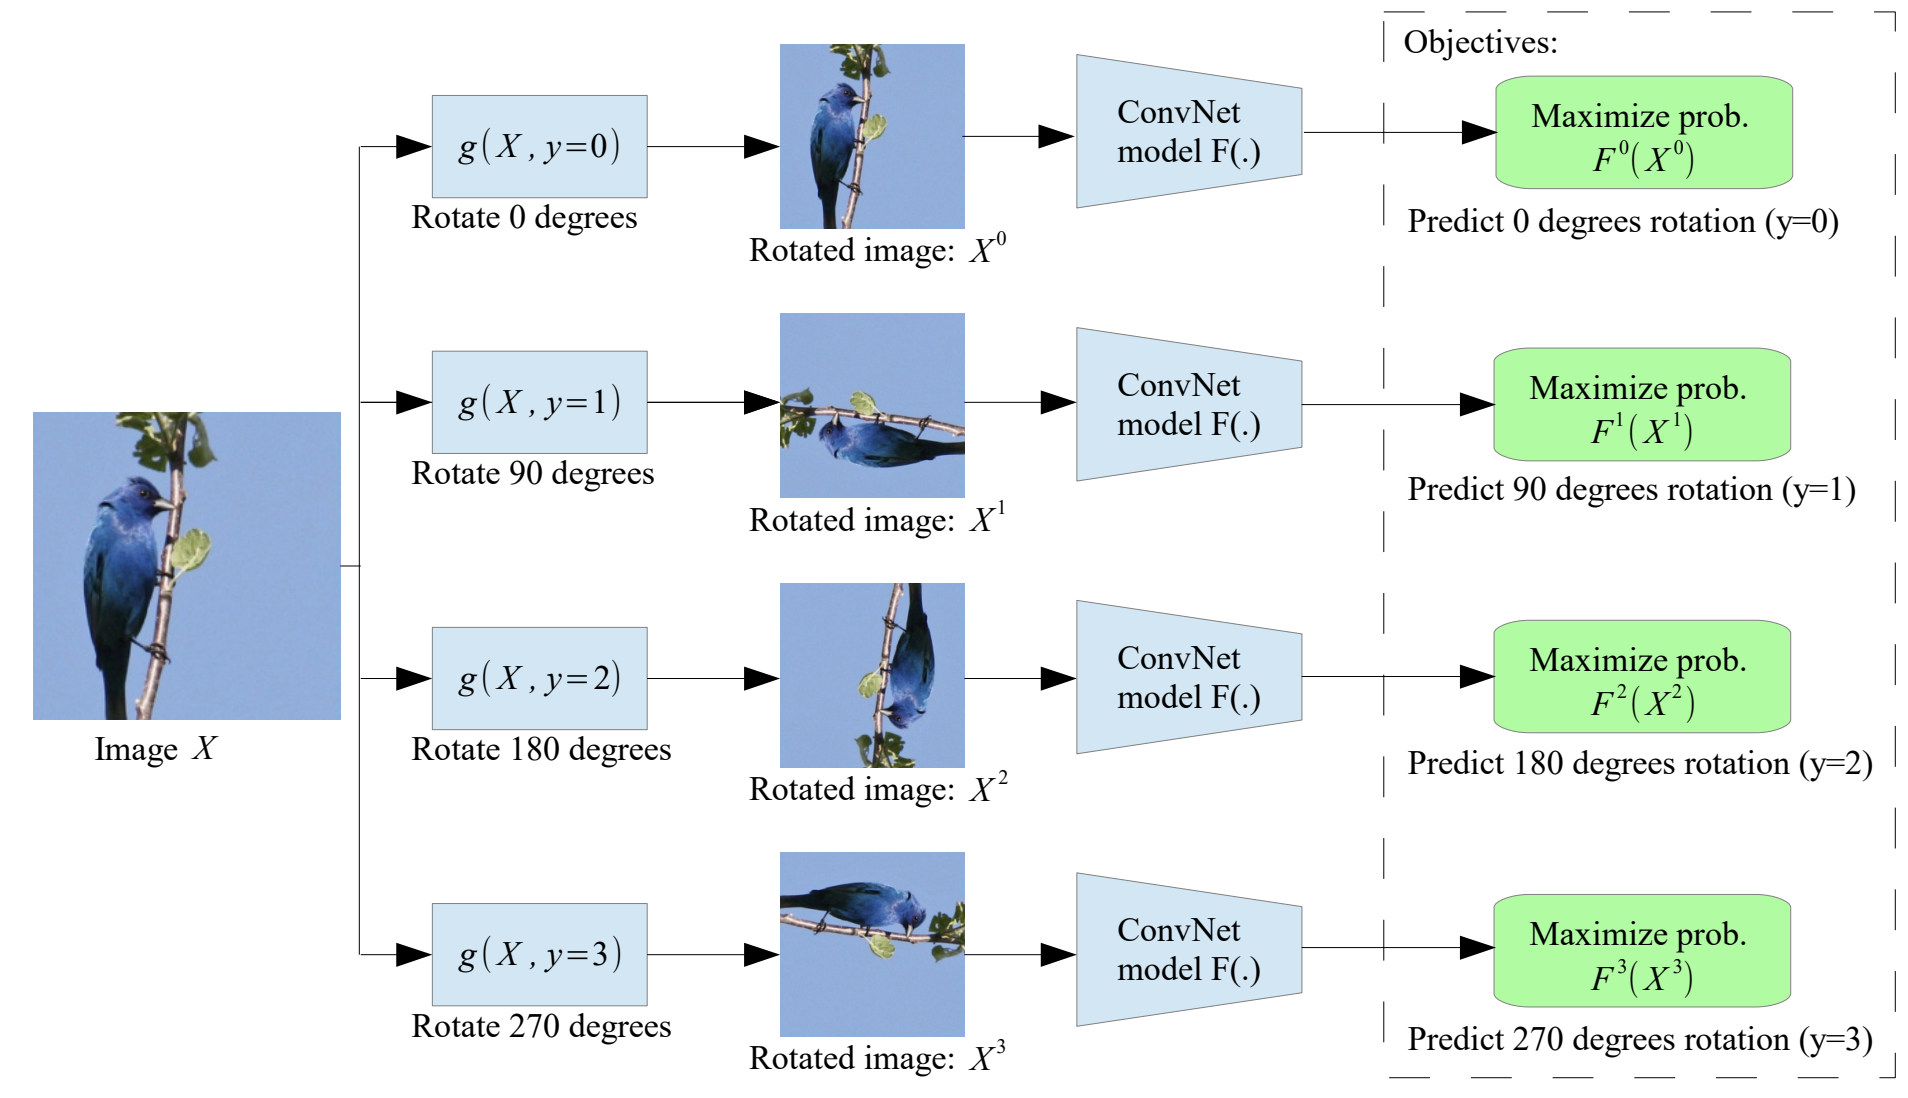
\includegraphics[width=1\linewidth,height=\textheight,keepaspectratio]{images/ssl/slide_33_1_img.png}
    \end{figure}

    \framebreak

    \begin{figure}
        \flushleft
        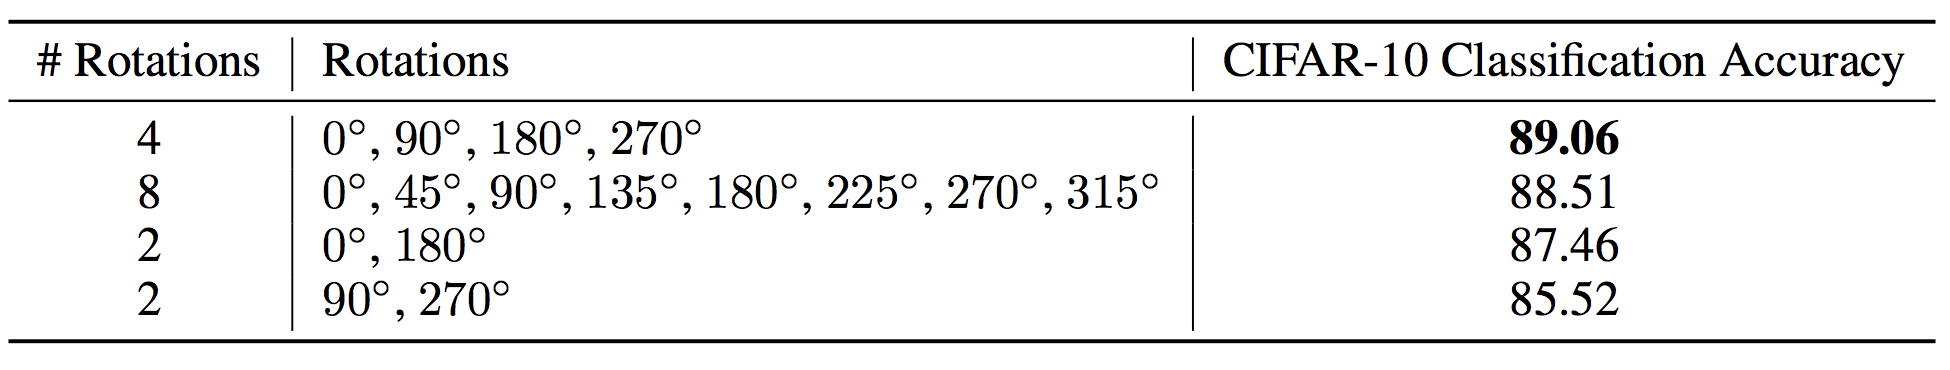
\includegraphics[width=1\linewidth,height=\textheight,keepaspectratio]{images/ssl/slide_34_1_img.png}
    \end{figure}

    \framebreak

    \textbf{Benefits:}
    \begin{itemize}
        \item Simple to implement and computationally inexpensive.
        \item Effective for learning global shape and semantic features.
        \item Can be used as a pretext task for downstream applications (e.g., image classification, object detection).
    \end{itemize}
    \textbf{References:}
    \begin{itemize}
        \item Gidaris, S., Singh, P., & Komodakis, N. (2018). Unsupervised Representation Learning by Predicting Image Rotations. \textit{ICLR 2018}.
    \end{itemize}
\end{frame}
% \begin{frame}[allowframebreaks]{Contrastive Predictive Coding (CPC)}
    \begin{figure}
        \centering
        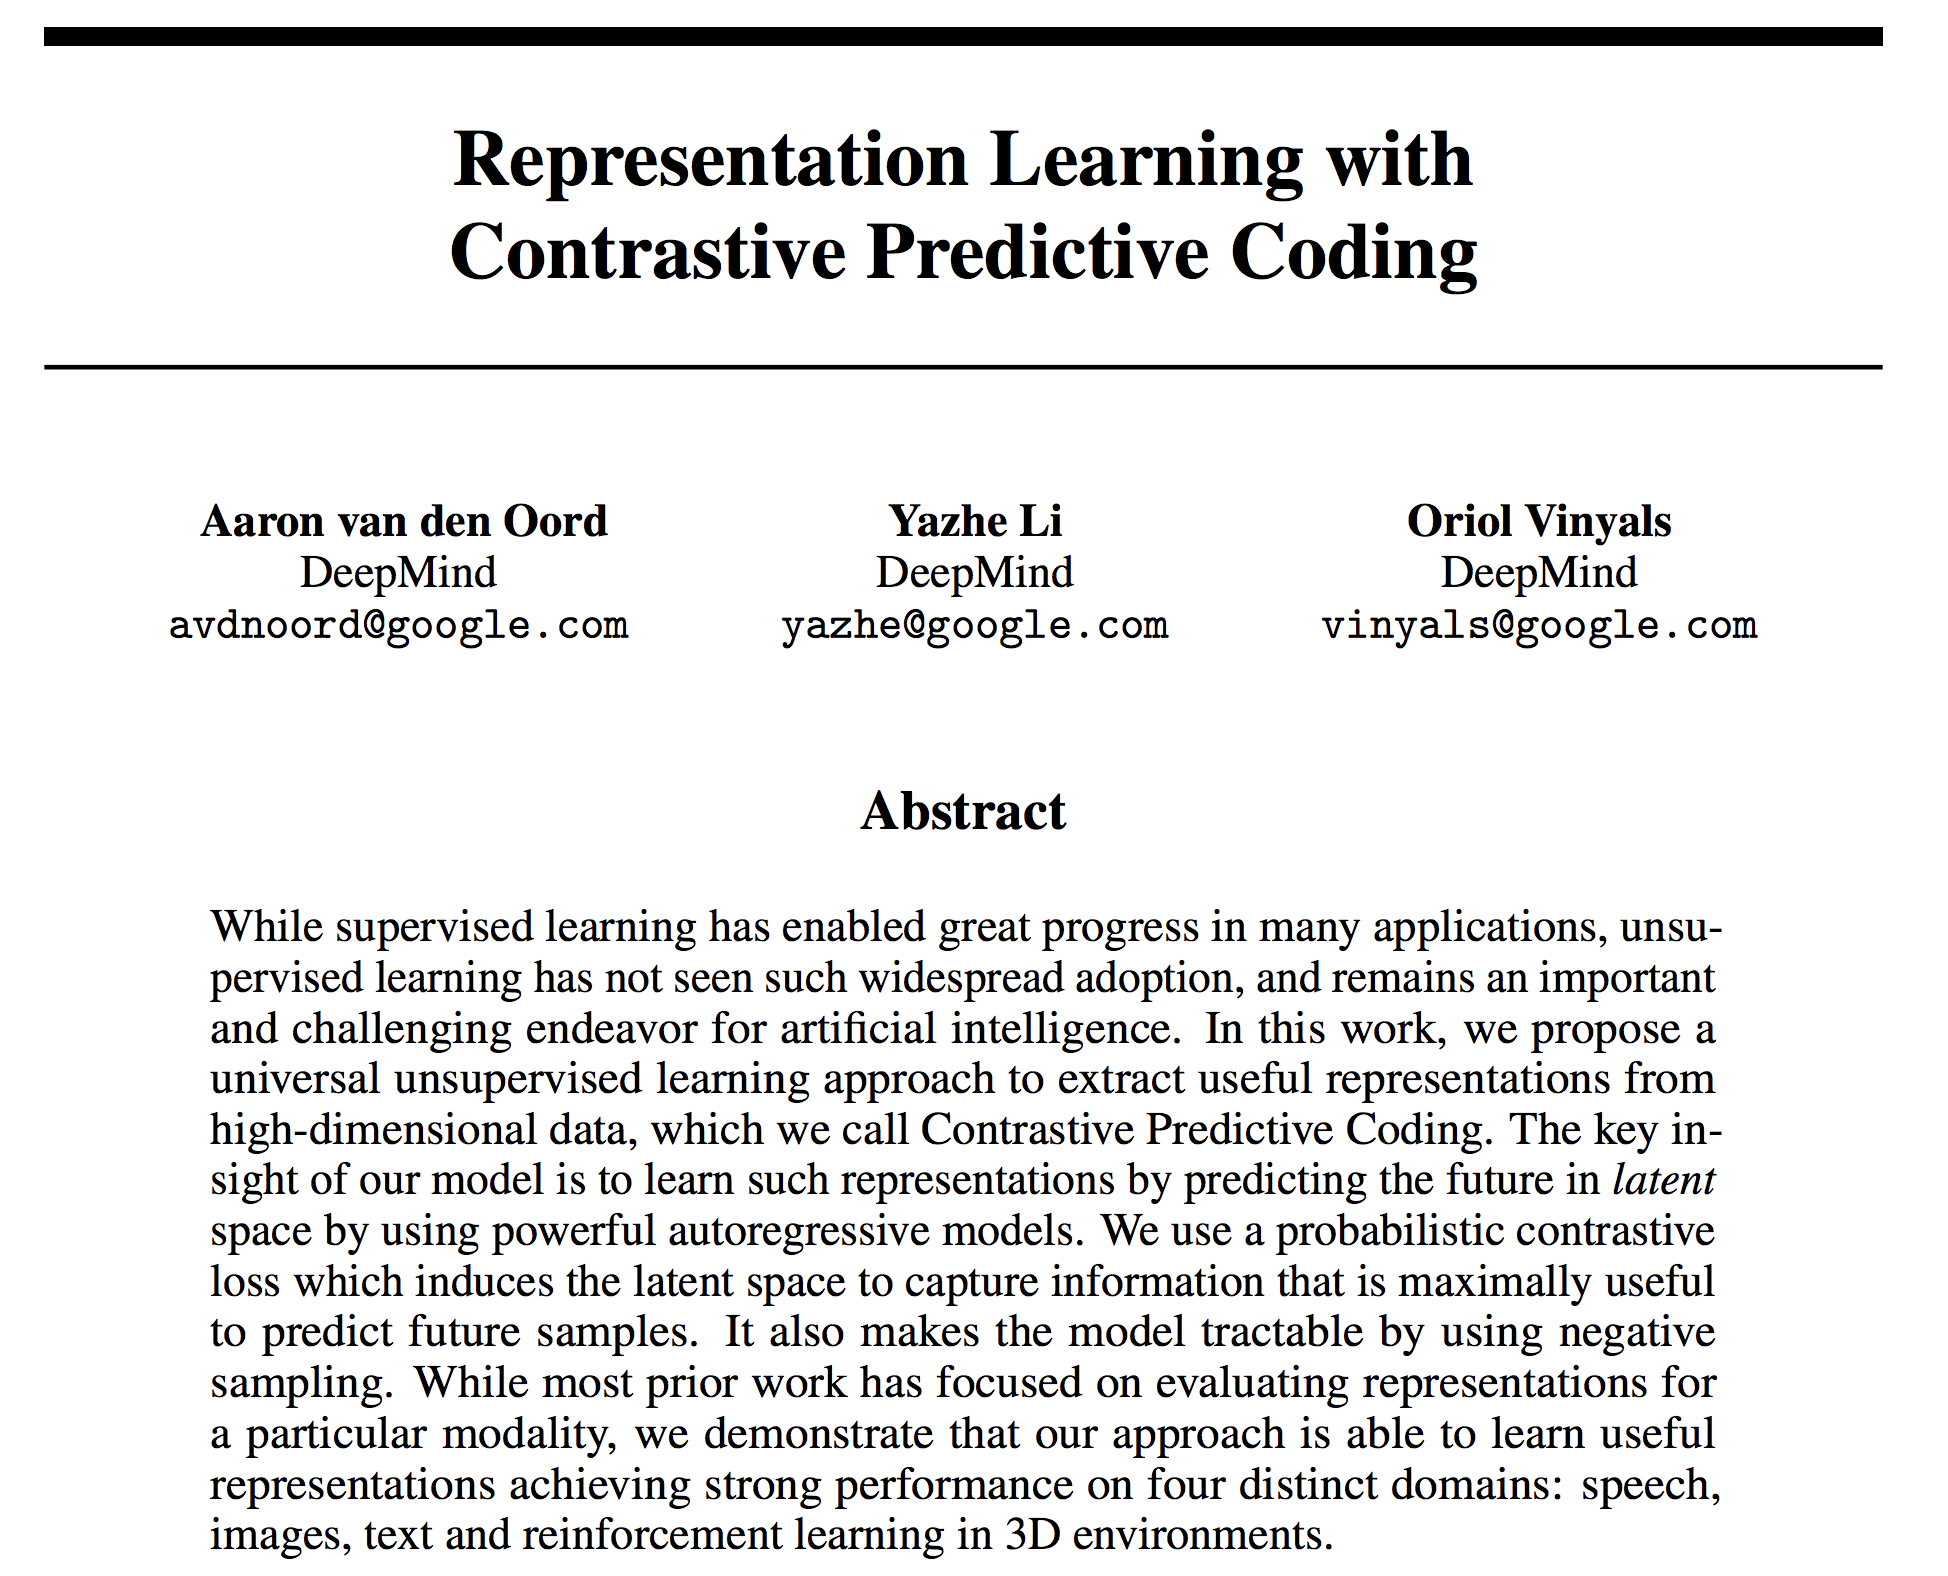
\includegraphics[width=1\linewidth,height=0.9\textheight,keepaspectratio]{images/ssl/slide_44_1_img.png}
    \end{figure}

    \framebreak

    \textbf{Contrastive Predictive Coding (CPC)} learns useful representations by predicting future information in latent space using powerful autoregressive models. The key components of CPC are:

    \begin{itemize}
        \item \textbf{Encoder}: Maps the input sequence $\mathbf{x}_t$ to a sequence of latent representations $\mathbf{z}_t$.
        \begin{itemize}
            \item Typically implemented as a convolutional or recurrent neural network.
            \item $\mathbf{z}_t = \text{Encoder}(\mathbf{x}_t)$
        \end{itemize}
        \item \textbf{Autoregressor}: Aggregates the sequence of past latents $\{\mathbf{z}_1, \ldots, \mathbf{z}_t\}$ into a context vector $\mathbf{c}_t$.
        \begin{itemize}
            \item Often implemented as an RNN or masked transformer.
            \item $\mathbf{c}_t = \text{AR}(\mathbf{z}_{\leq t})$
        \end{itemize}
        \item \textbf{Prediction}: The model predicts future latent representations using the context vector.
        \begin{itemize}
            \item For each step $k$, a linear transformation $W_k$ is applied to the context: $\hat{\mathbf{z}}_{t+k} = W_k \mathbf{c}_t$
            \item The goal is to distinguish the true future latent $\mathbf{z}_{t+k}$ from negative samples.
        \end{itemize}
        \item \textbf{InfoNCE Loss}: A contrastive loss that encourages the predicted future latent to be similar to the true future latent and dissimilar to negative samples.
        \begin{itemize}
            \item For each prediction step $k$:
            \[
                \mathcal{L}_{\text{InfoNCE}} = -\mathbb{E} \left[ \log \frac{\exp(\mathbf{z}_{t+k}^\top W_k \mathbf{c}_t)}{\sum\limits_{j} \exp(\mathbf{z}_j^\top W_k \mathbf{c}_t)} \right]
            \]
            \item The denominator sums over one positive and multiple negative samples.
        \end{itemize}
    \end{itemize}

    \framebreak

    \begin{figure}
        \centering
        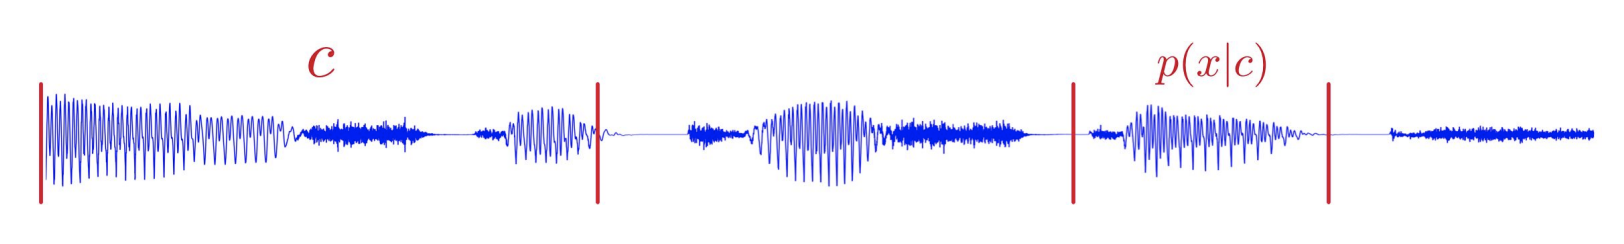
\includegraphics[width=1\linewidth,height=0.9\textheight,keepaspectratio]{images/ssl/slide_45_1_img.png}
    \end{figure}

    \framebreak

    \begin{figure}
        \centering
        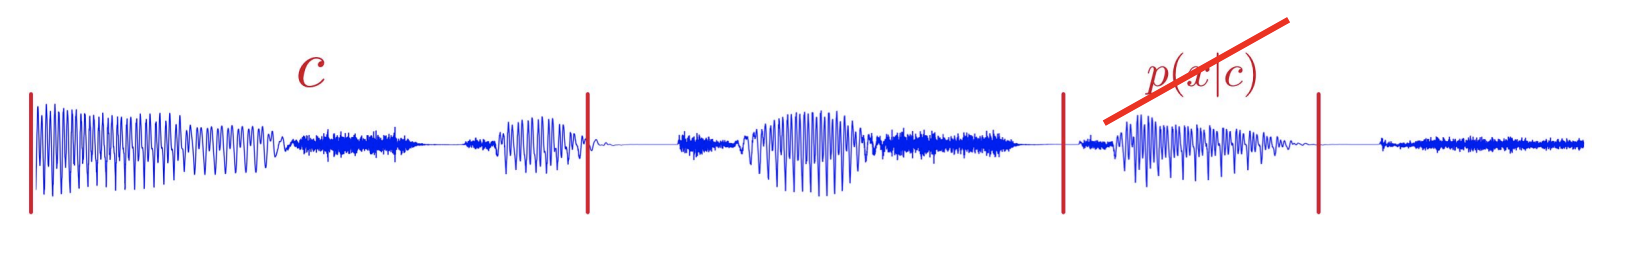
\includegraphics[width=1\linewidth,height=0.9\textheight,keepaspectratio]{images/ssl/slide_46_2_img.png}
    \end{figure}

    \framebreak

    \begin{figure}
        \centering
        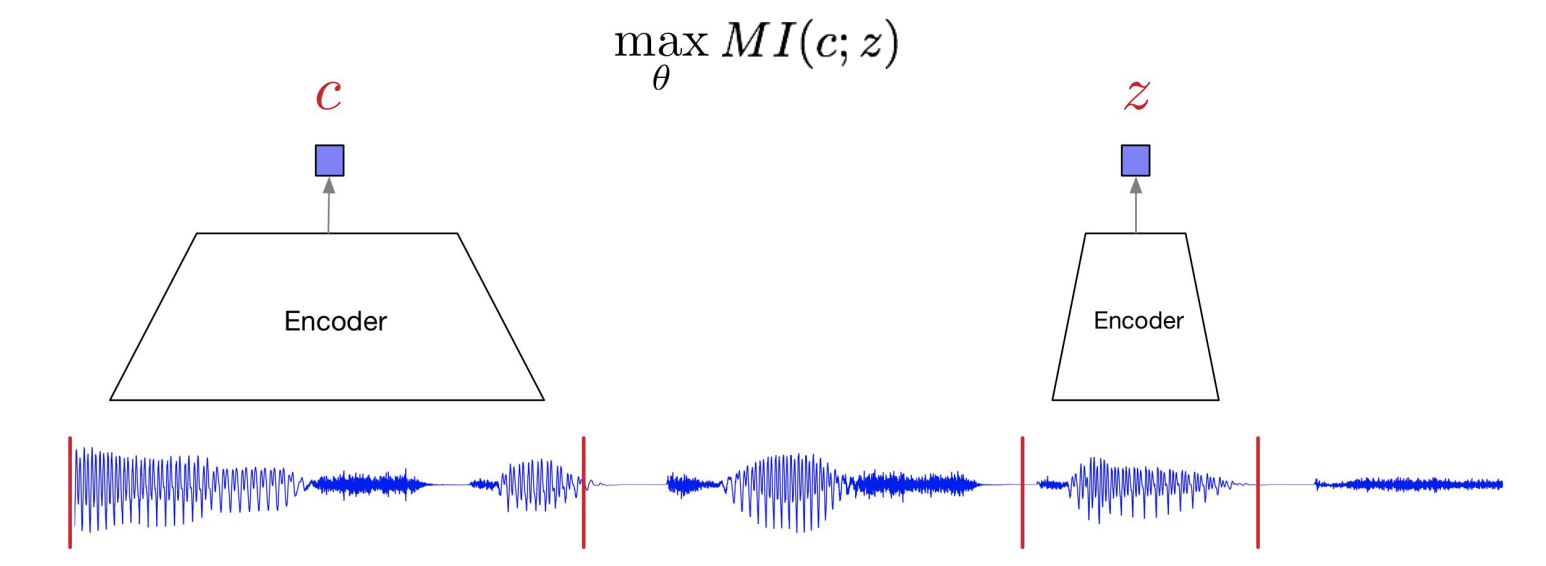
\includegraphics[width=1\linewidth,height=0.9\textheight,keepaspectratio]{images/ssl/slide_47_3_img.png}
    \end{figure}

    \framebreak

    \begin{figure}
        \centering
        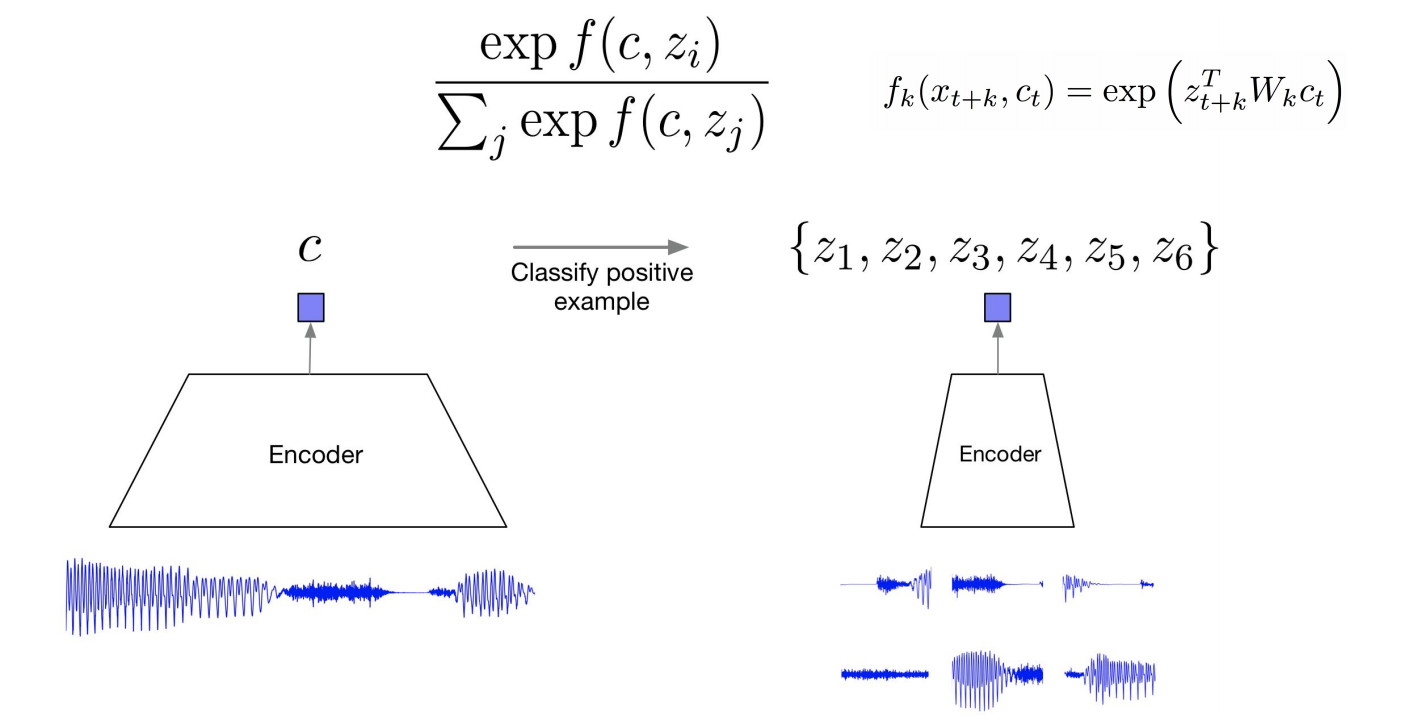
\includegraphics[width=1\linewidth,height=0.9\textheight,keepaspectratio]{images/ssl/slide_48_4_img.png}
    \end{figure}

    \framebreak

    \begin{figure}
        \centering
        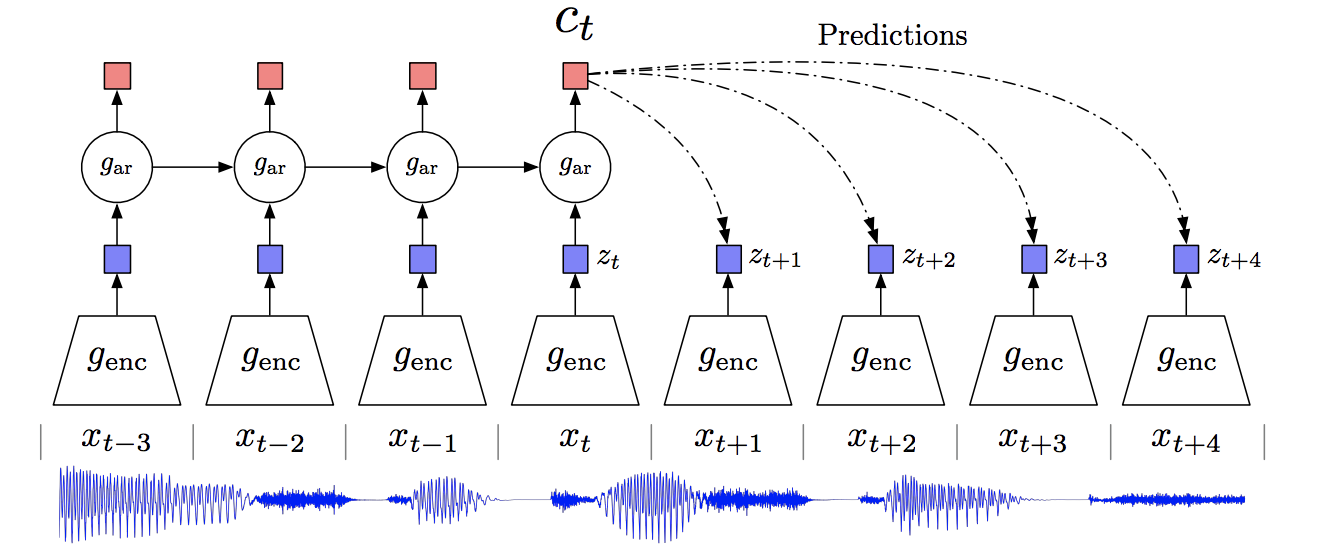
\includegraphics[width=1\linewidth,height=0.9\textheight,keepaspectratio]{images/ssl/slide_49_1_img.png}
    \end{figure}

    \framebreak

    \begin{figure}
        \centering
        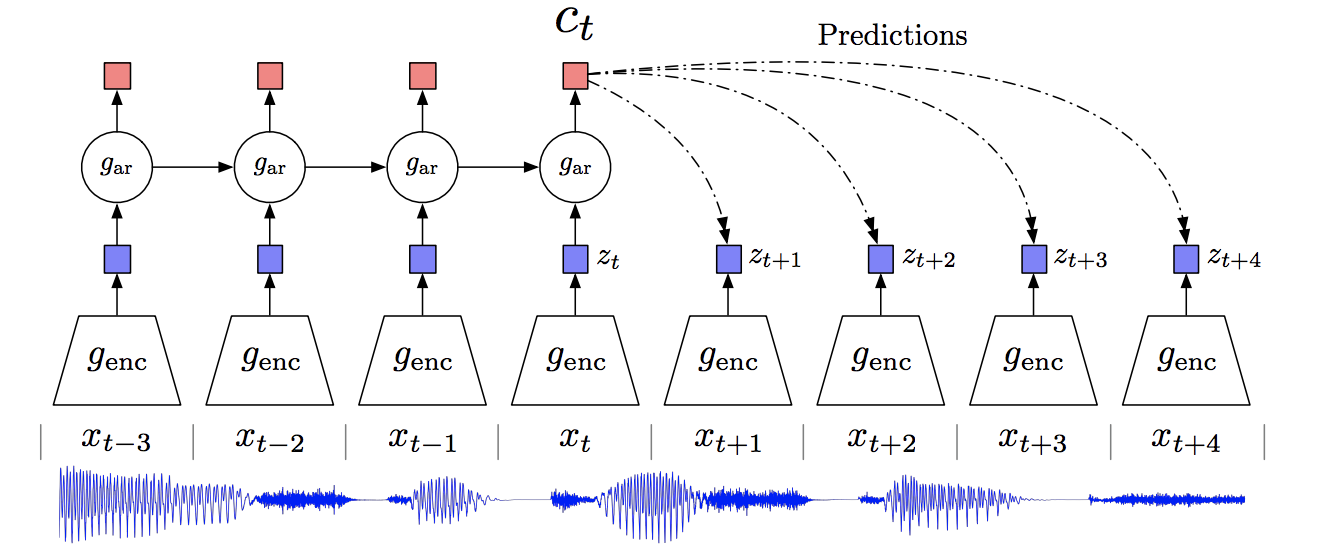
\includegraphics[width=1\linewidth,height=0.5\textheight,keepaspectratio]{images/ssl/slide_50_2_img.png}
    \end{figure}

    \begin{figure}
        \centering
        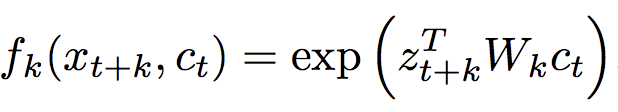
\includegraphics[width=0.5\linewidth,height=0.3\textheight,keepaspectratio]{images/ssl/slide_50_3_img.png}
    \end{figure}

    \begin{figure}
        \centering
        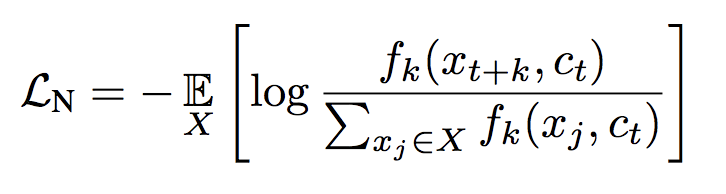
\includegraphics[width=0.5\linewidth,height=0.3\textheight,keepaspectratio]{images/ssl/slide_50_1_img.png}
    \end{figure}

    \framebreak

    \textbf{Key Points about CPC}:
    \begin{itemize}
        \item CPC learns representations by maximizing mutual information between context and future latent representations.
        \item It is widely used in audio, vision, and language domains for self-supervised pretraining.
        \item The contrastive loss enables learning without explicit labels, relying on the structure of the data itself.
    \end{itemize}
\end{frame}

\begin{frame}[allowframebreaks]{CPC: Speech}
    \begin{columns}
        \column{0.5\textwidth}
        \begin{figure}
            \centering
            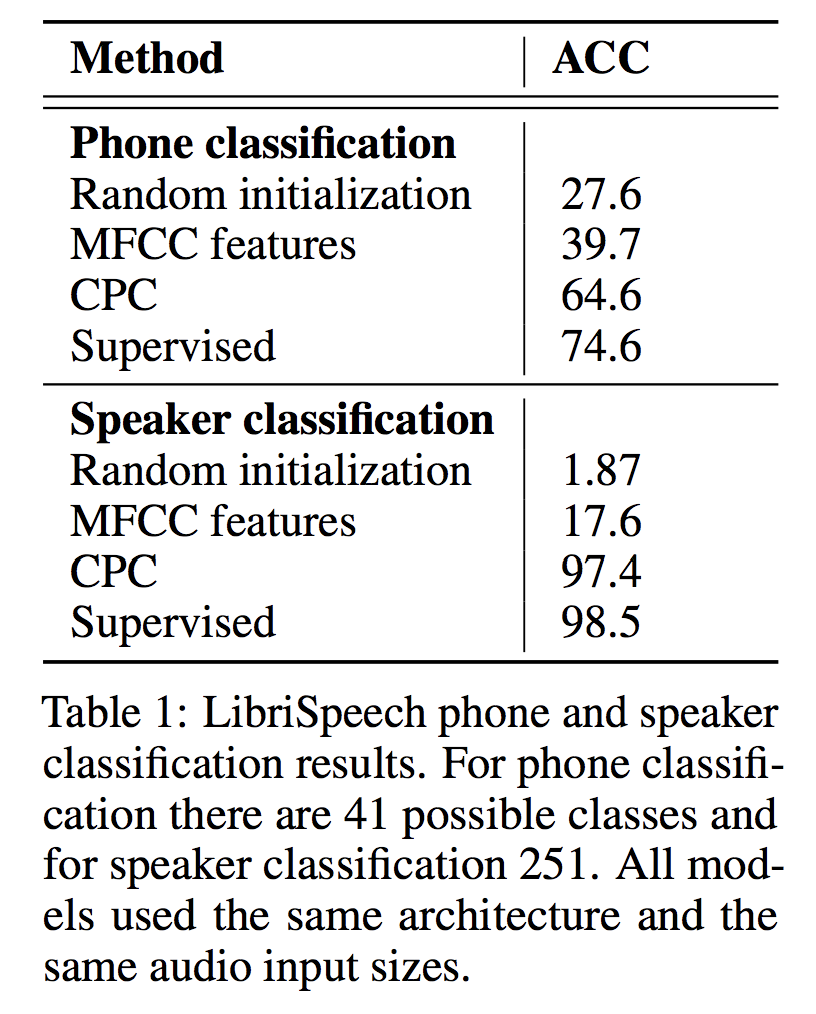
\includegraphics[width=1\linewidth,height=0.9\textheight,keepaspectratio]{images/ssl/slide_52_1_img.png}
        \end{figure}

        \column{0.5\textwidth}
        \begin{figure}
            \centering
            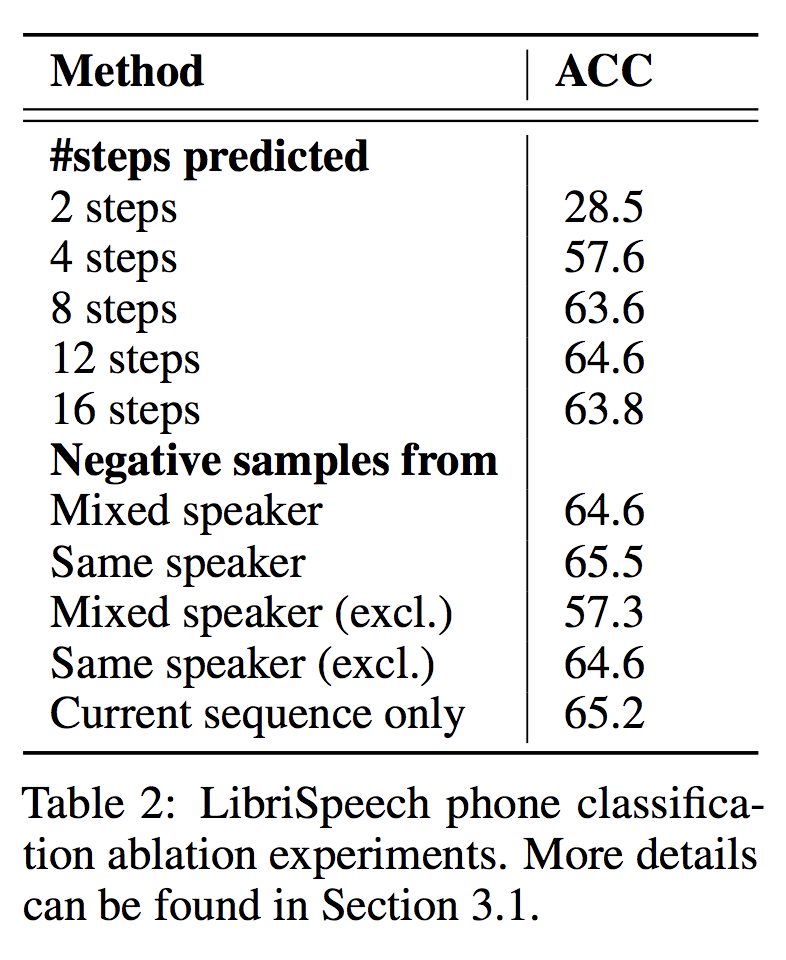
\includegraphics[width=1\linewidth,height=0.9\textheight,keepaspectratio]{images/ssl/slide_52_2_img.png}
        \end{figure}
    \end{columns}
\end{frame}

\begin{frame}[allowframebreaks]{CPC: ImageNet}
    \begin{figure}
        \centering
        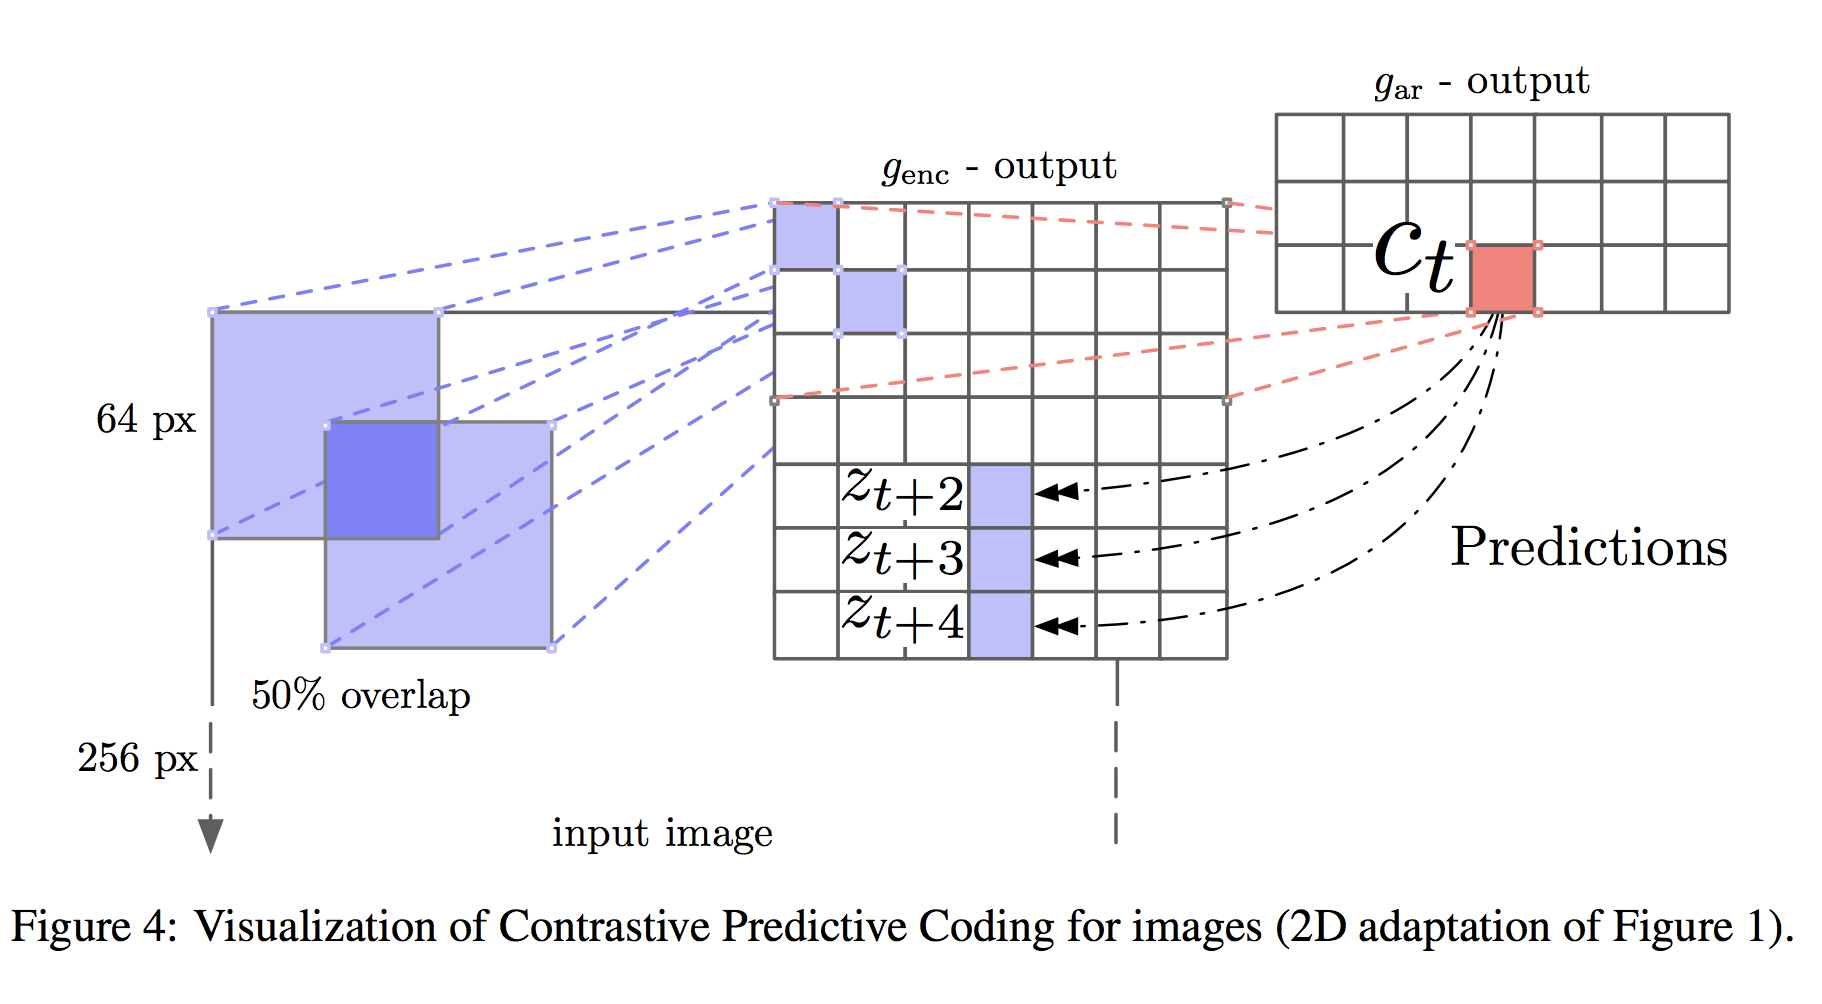
\includegraphics[width=1\linewidth,height=0.9\textheight,keepaspectratio]{images/ssl/slide_53_1_img.png}
    \end{figure}

    \framebreak

    \begin{columns}
        \column{0.5\textwidth}
        \begin{figure}
            \centering
            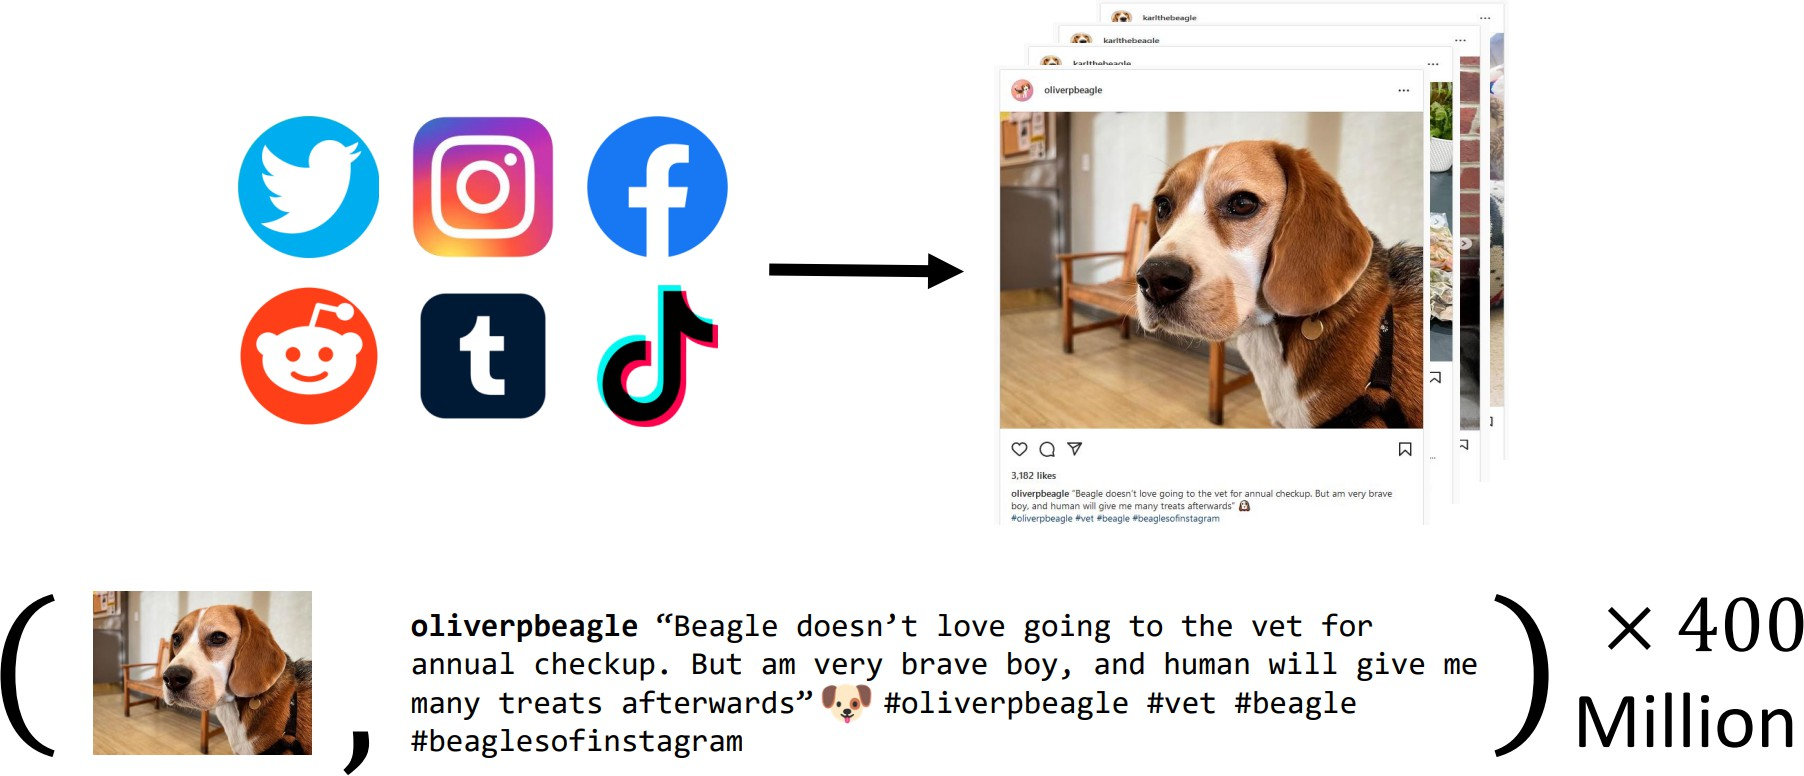
\includegraphics[width=1\linewidth,height=0.9\textheight,keepaspectratio]{images/ssl/slide_54_1_img.png}
        \end{figure}

        \column{0.5\textwidth}
        \begin{figure}
            \centering
            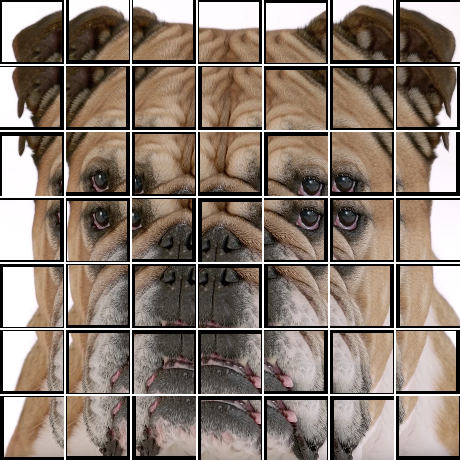
\includegraphics[width=1\linewidth,height=0.9\textheight,keepaspectratio]{images/ssl/slide_54_2_img.png}
        \end{figure}
    \end{columns}

    \framebreak

    \begin{figure}
        \centering
        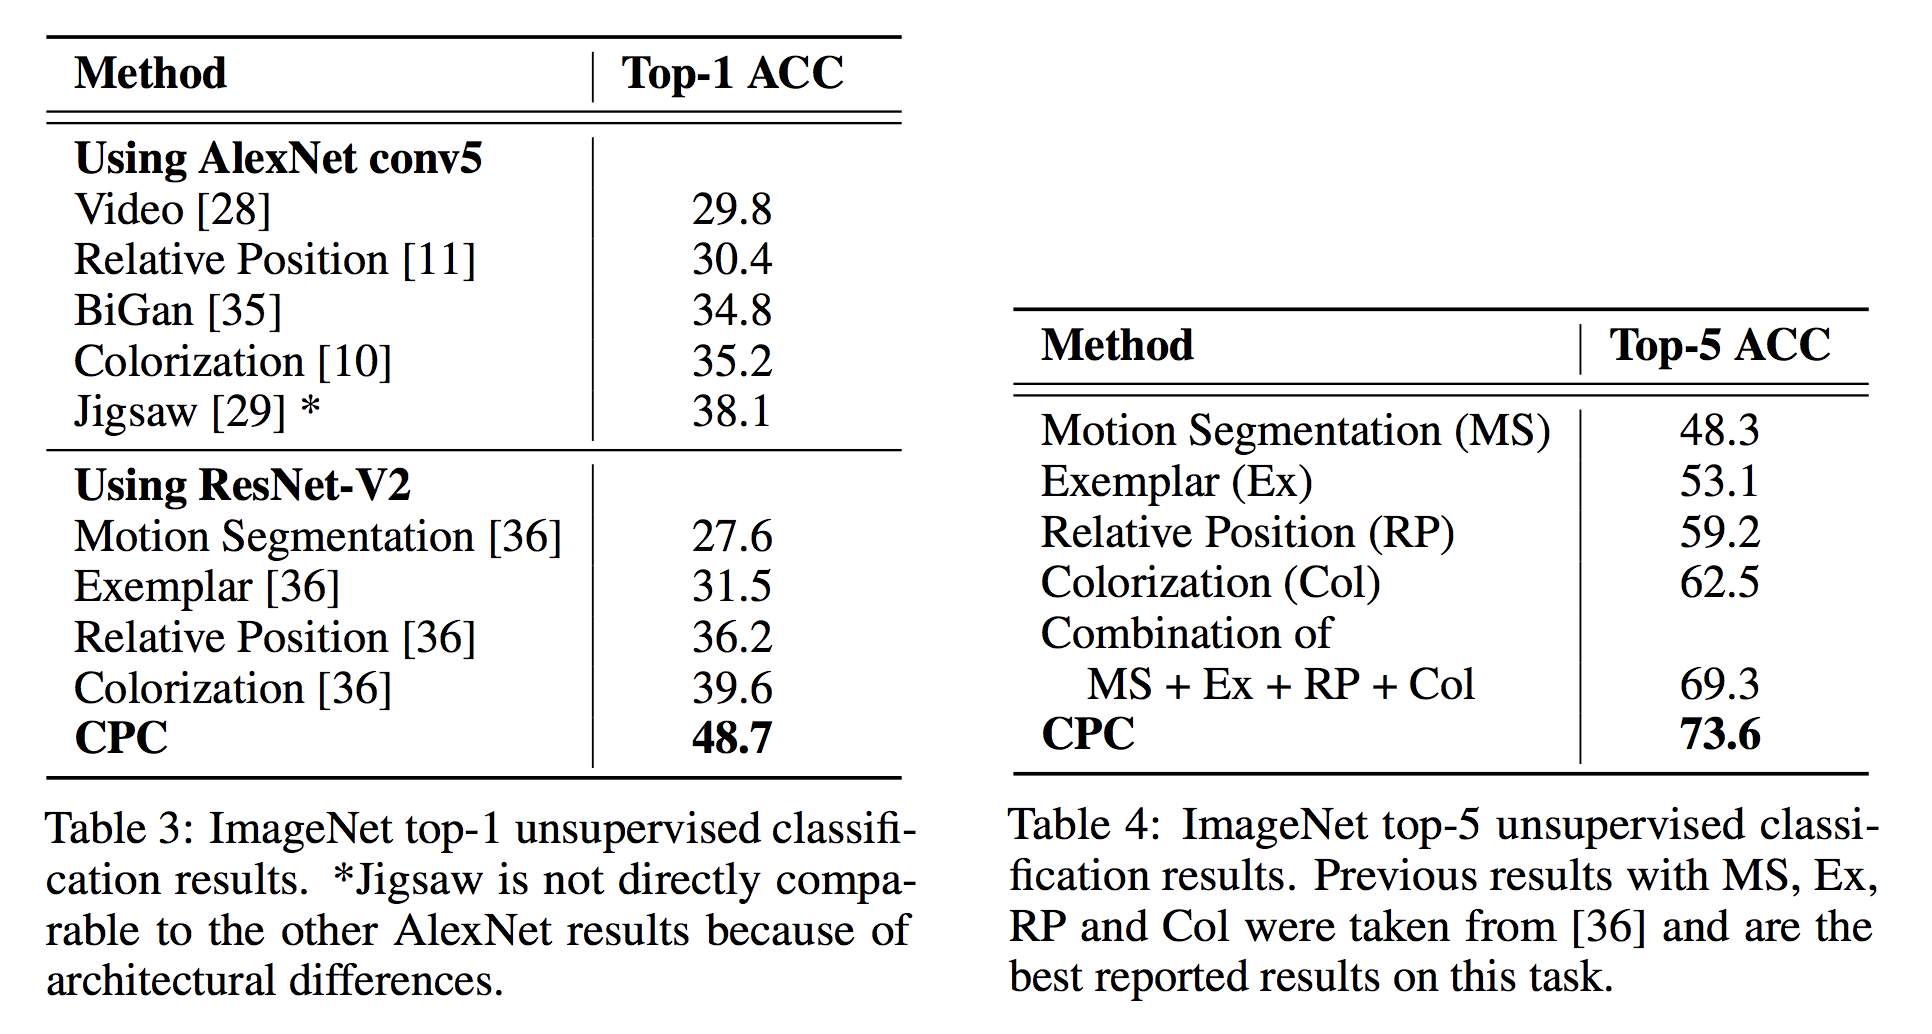
\includegraphics[width=1\linewidth,height=0.9\textheight,keepaspectratio]{images/ssl/slide_55_1_img.png}
    \end{figure}

    \framebreak

    \begin{figure}
        \centering
        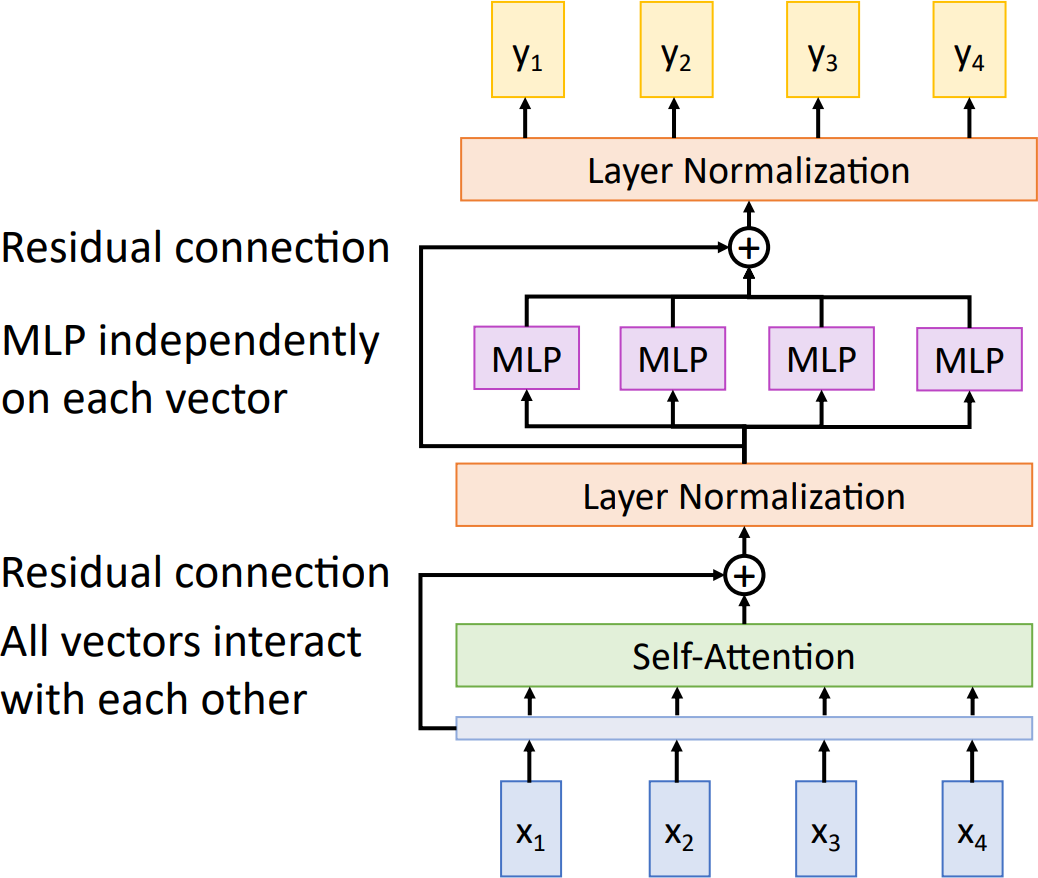
\includegraphics[width=1\linewidth,height=0.9\textheight,keepaspectratio]{images/ssl/slide_56_1_img.png}
    \end{figure}
\end{frame}


\begin{frame}[allowframebreaks]{CPC: Natural Language Processing}
    \begin{figure}
        \centering
        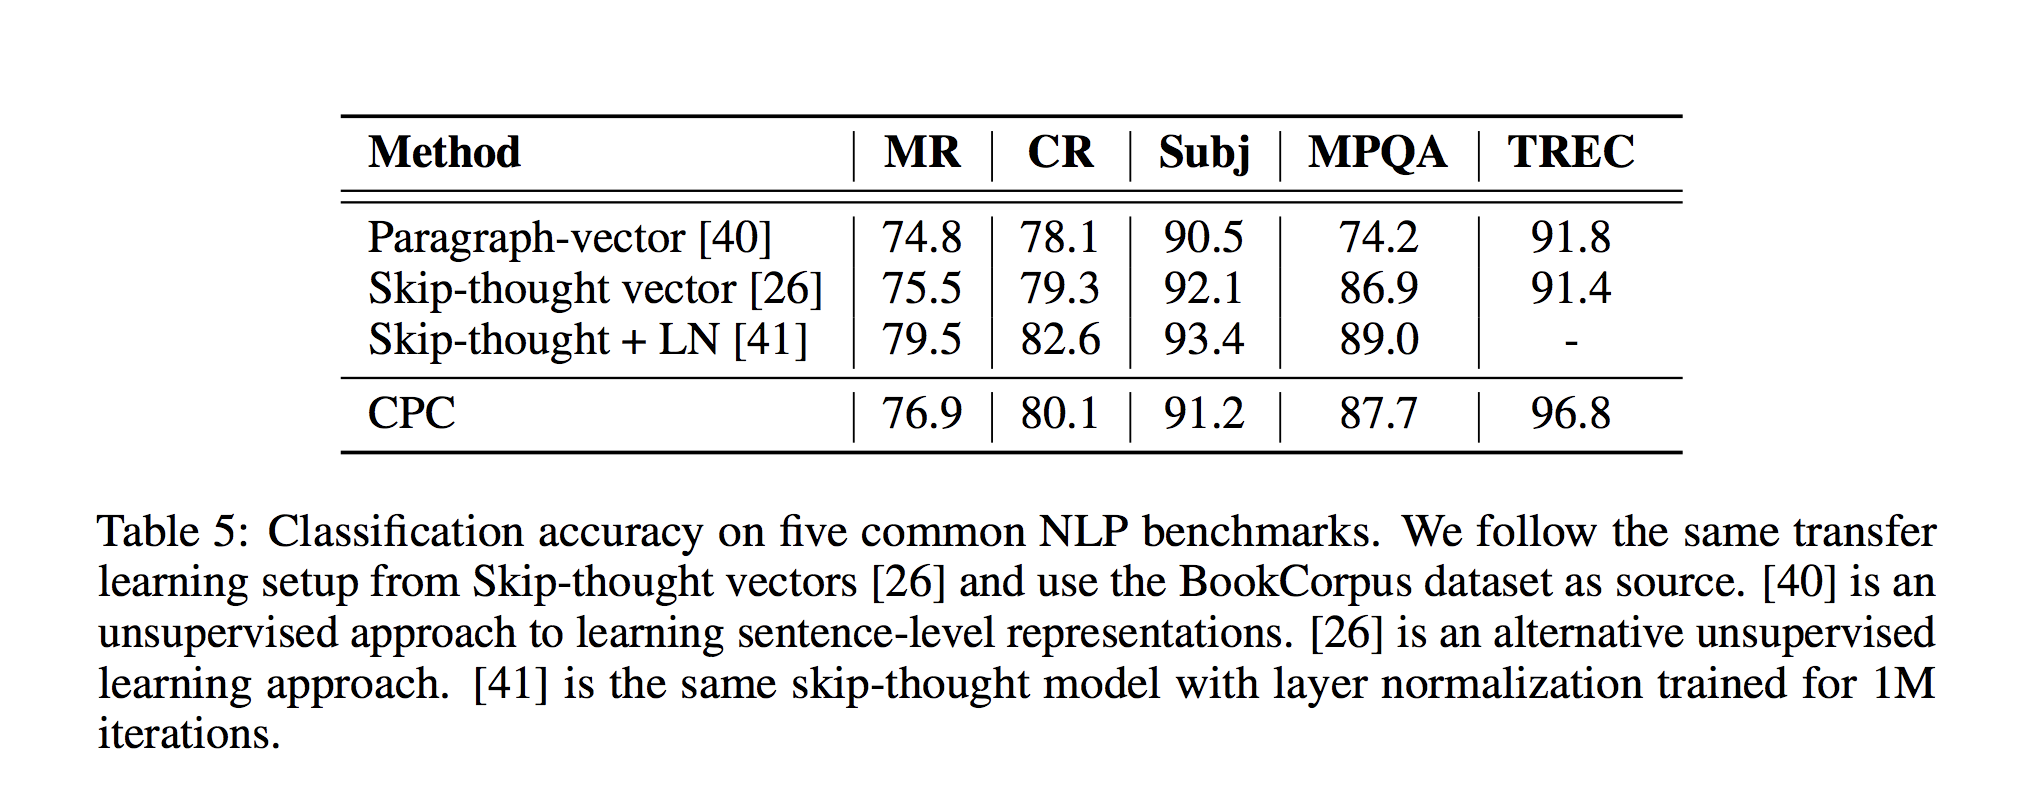
\includegraphics[width=1\linewidth,height=0.9\textheight,keepaspectratio]{images/ssl/slide_57_1_img.png}
    \end{figure}
\end{frame}


\begin{frame}[allowframebreaks]{CPC: Reinforcement Learning}
    \begin{figure}
        \centering
        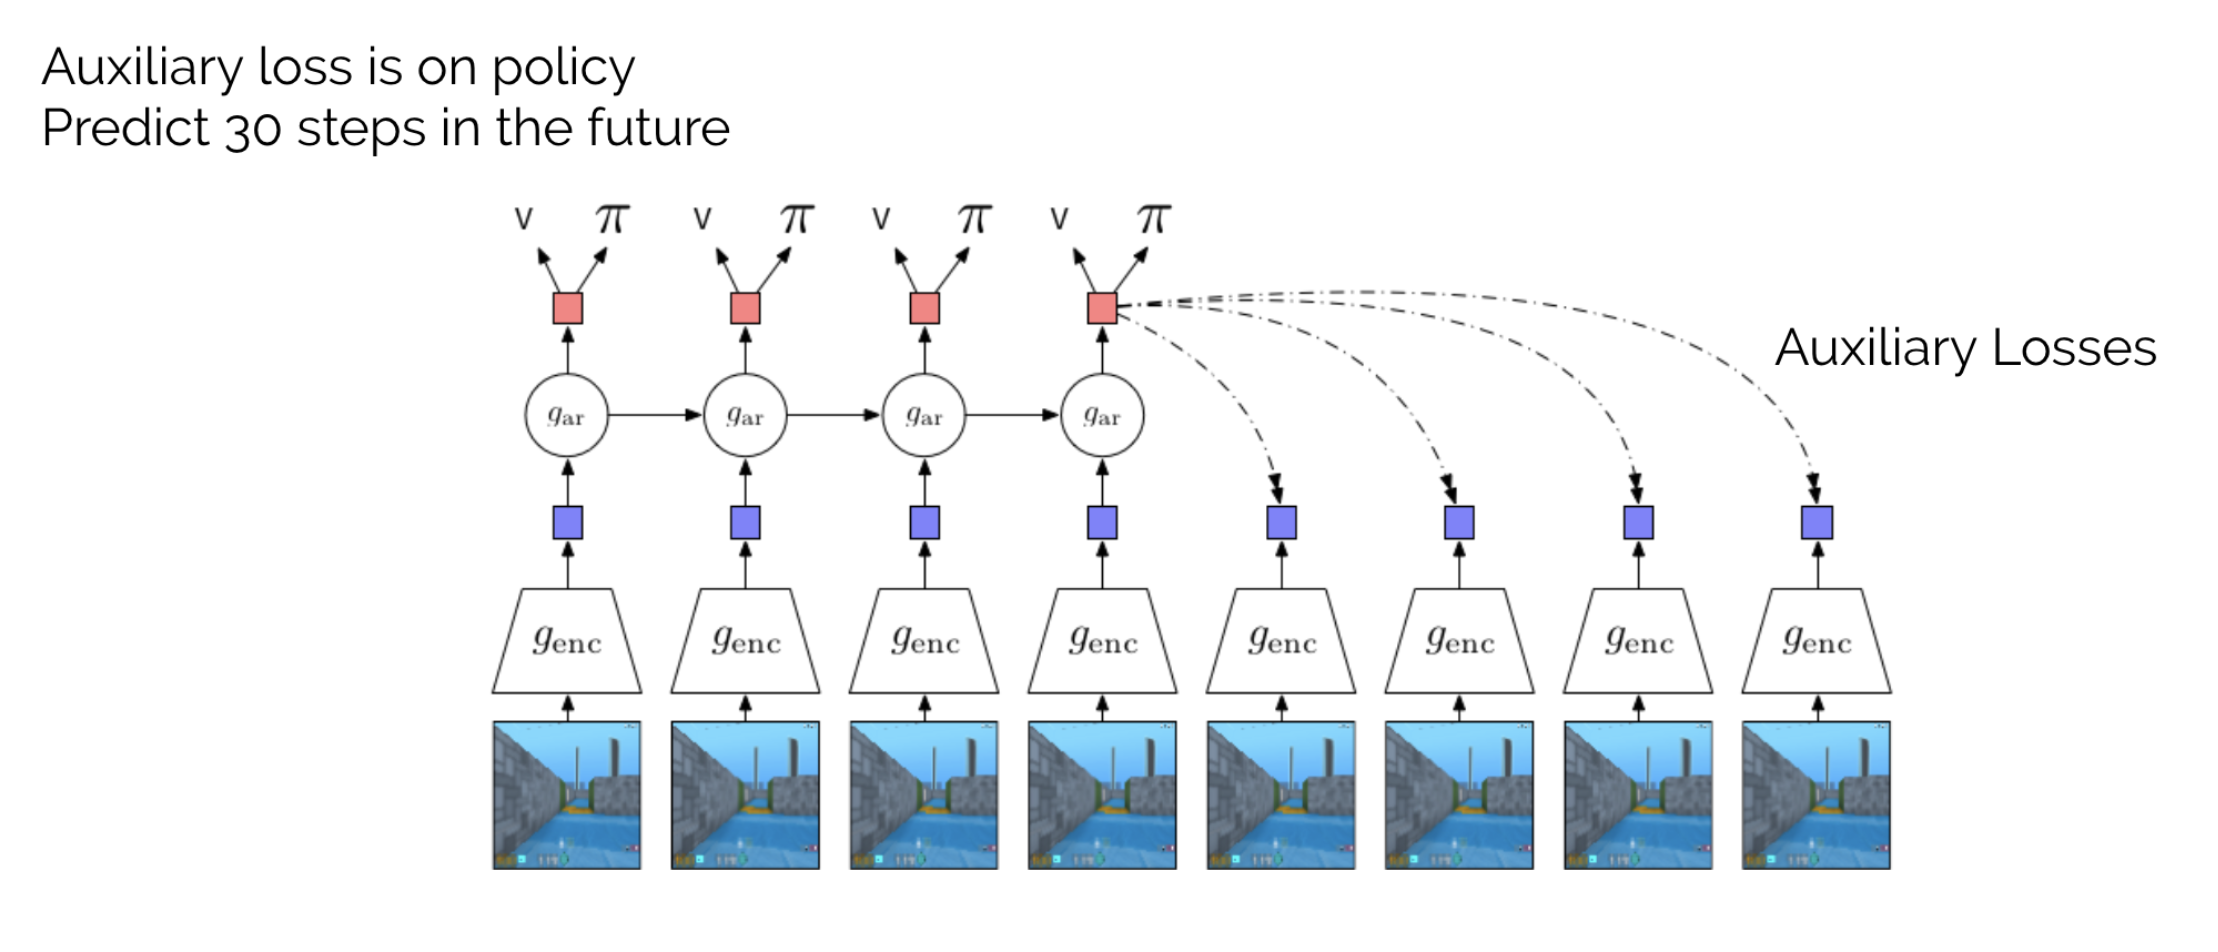
\includegraphics[width=1\linewidth,height=0.9\textheight,keepaspectratio]{images/ssl/slide_58_1_img.png}
    \end{figure}
\end{frame}


\begin{frame}[allowframebreaks]{CPCv2: Large Scale CPC on ImageNet}
    \begin{figure}
        \centering
        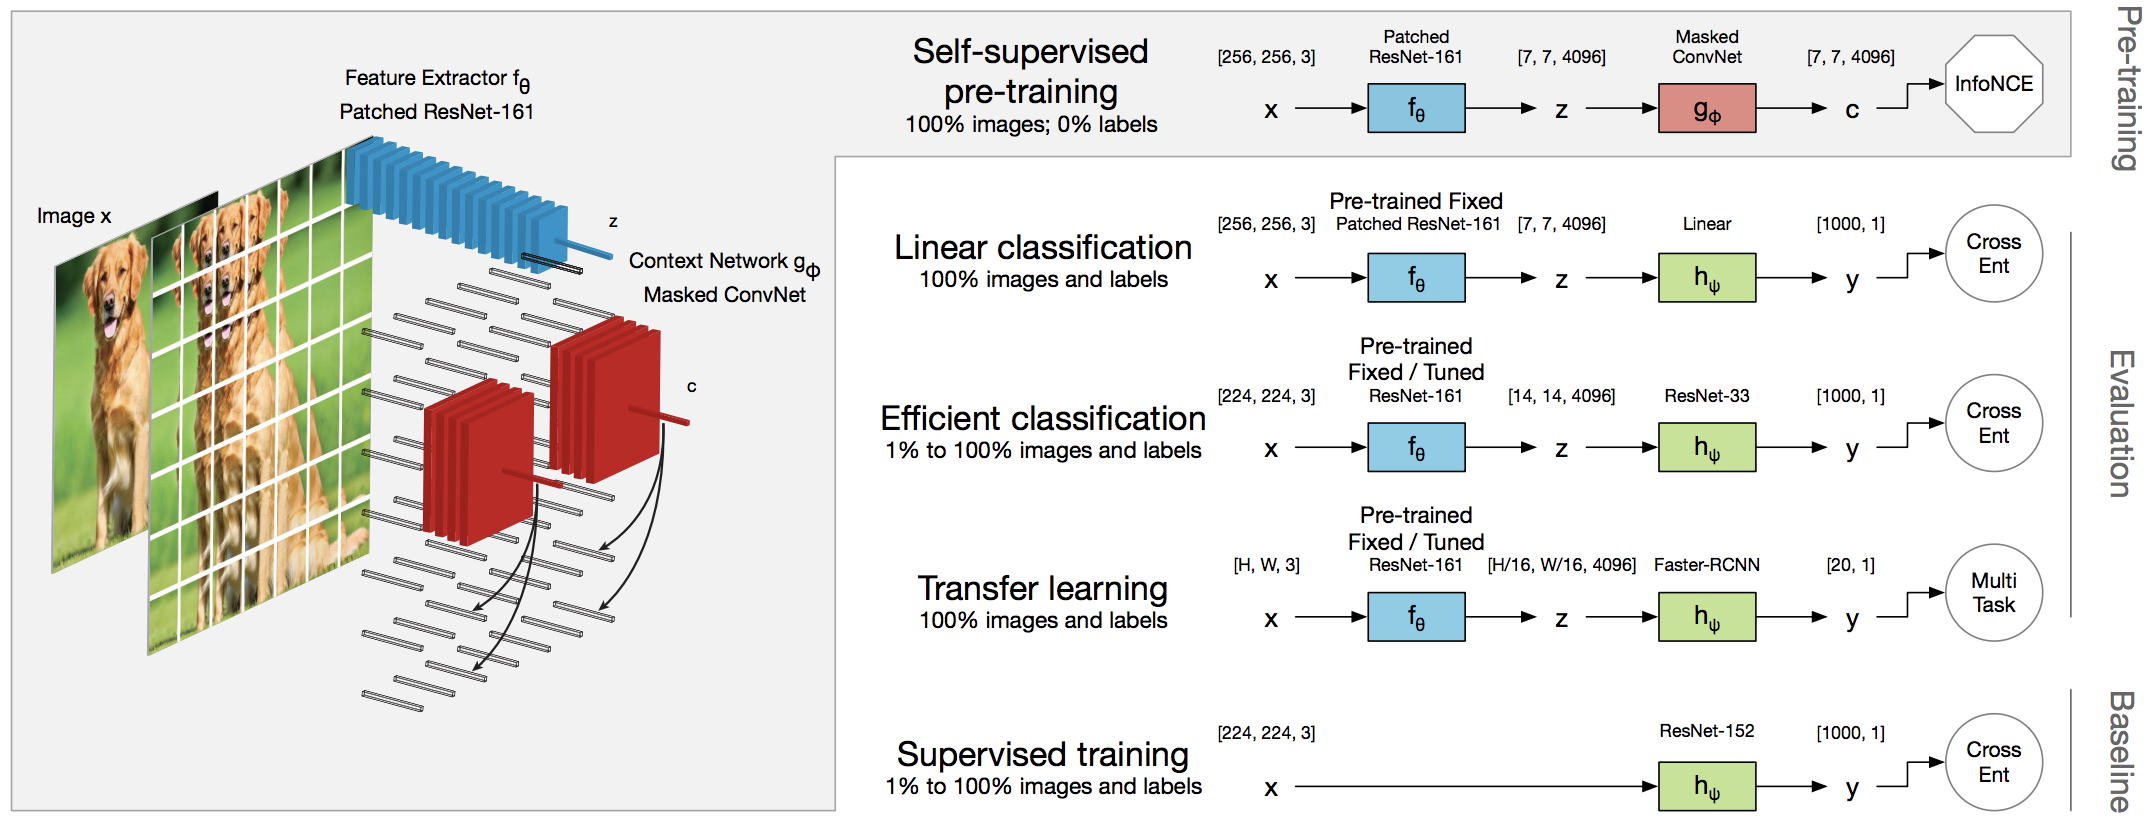
\includegraphics[width=1\linewidth,height=0.9\textheight,keepaspectratio]{images/ssl/slide_59_1_img.png}
    \end{figure}
\end{frame}

\begin{frame}[allowframebreaks]{CPCv2: Linear Classification}
    \begin{figure}
        \centering
        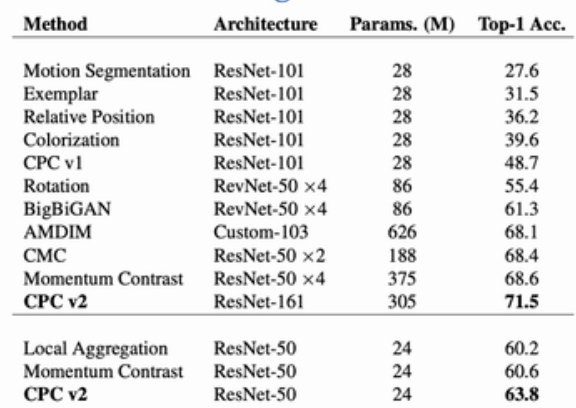
\includegraphics[width=1\linewidth,height=0.9\textheight,keepaspectratio]{images/ssl/slide_60_1_img.png}
    \end{figure}
\end{frame}


\begin{frame}[allowframebreaks]{CPCv2: Data-Efficient Image Recognition}
    \begin{figure}
        \centering
        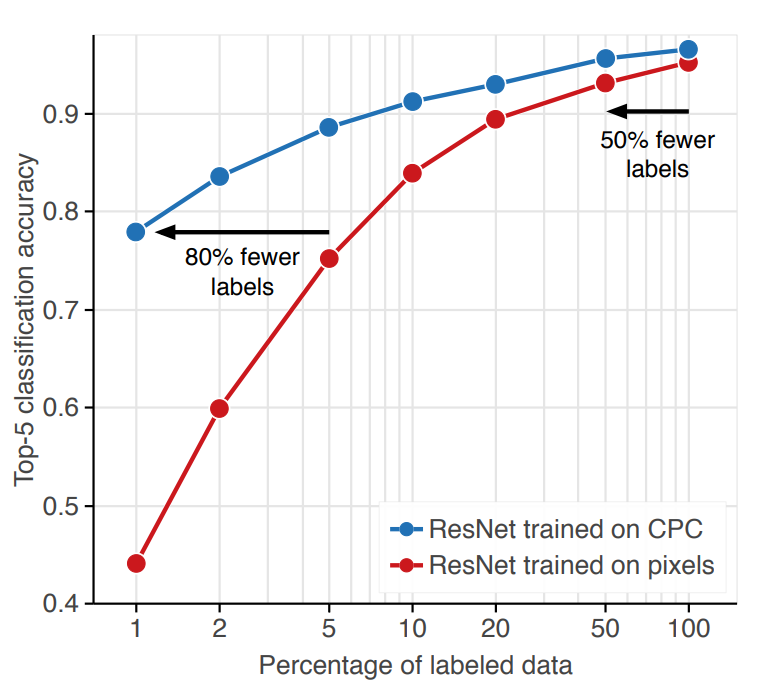
\includegraphics[width=1\linewidth,height=0.9\textheight,keepaspectratio]{images/ssl/slide_61_1_img.png}
    \end{figure}
\end{frame}


\begin{frame}[allowframebreaks]{CPCv2: Data-Efficient Supervised Learning}
    \begin{figure}
        \centering
        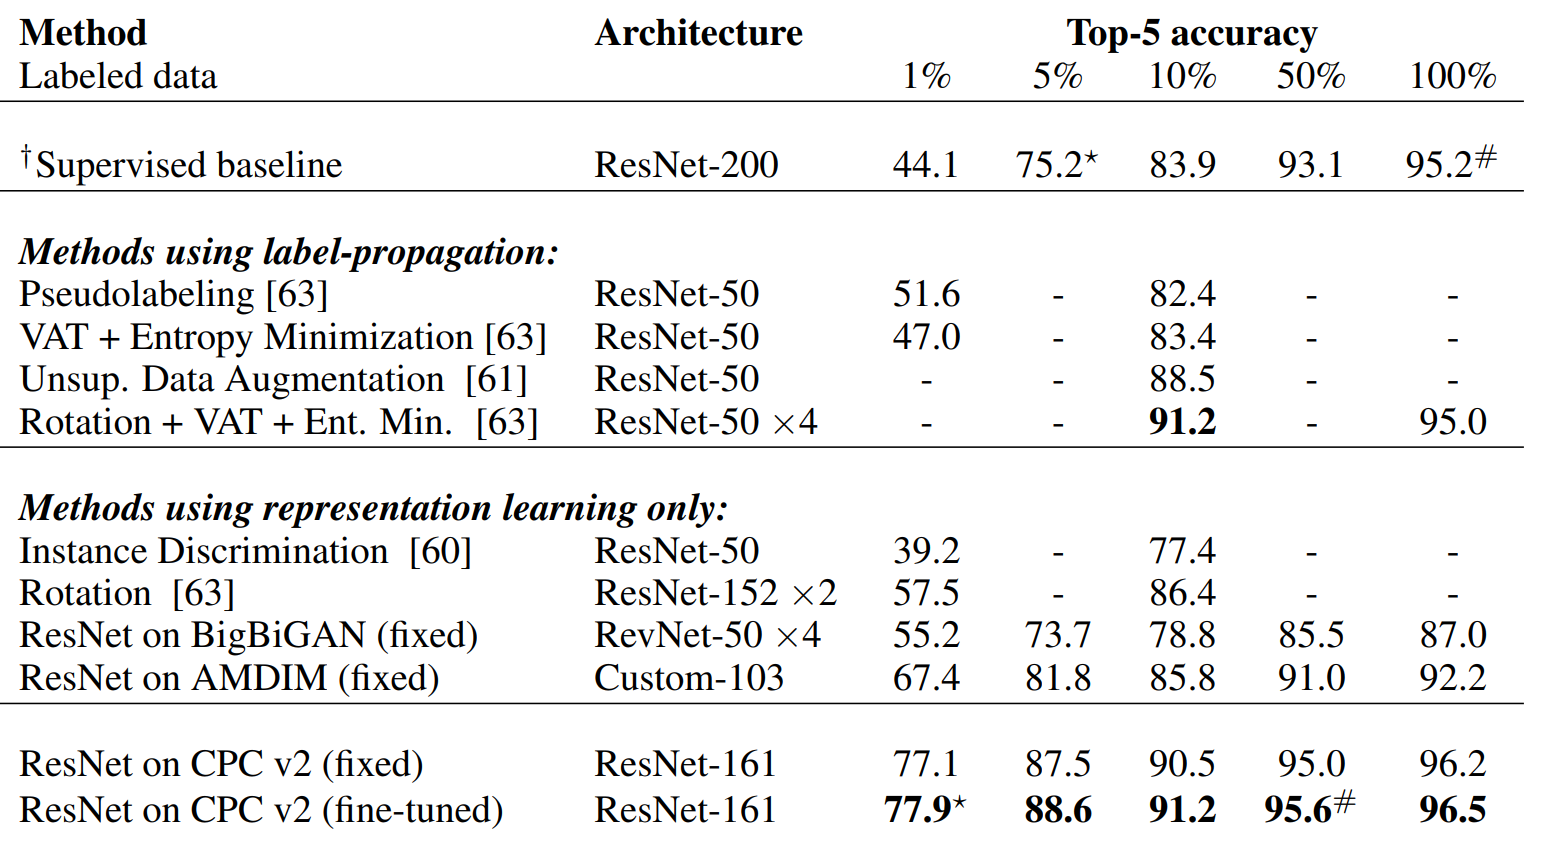
\includegraphics[width=1\linewidth,height=0.9\textheight,keepaspectratio]{images/ssl/slide_62_1_img.png}
    \end{figure}
\end{frame}
